%% This document is created by 
%%  Dr. Putu Harry Gunawan
%% Template untuk Proposal TA 1 dan TA
%% Template ini digunakan untuk penulisan proposal TA 1 atau TA Fakultas Informatika, Telkom University.

\documentclass[a4paper,12pt,oneside]{book}
\usepackage[utf8]{inputenc}
\usepackage{sectsty}
\usepackage{graphicx}
\usepackage{epstopdf}
\usepackage{algorithm}
\usepackage{algpseudocode}
\usepackage{array}
\usepackage[table]{xcolor}
\usepackage{anysize}
\usepackage{amsmath}
\usepackage{amssymb}
\usepackage[english]{babel}
\usepackage{indentfirst} %Spasi untuk paragraf pertama
\usepackage{geometry}
\usepackage{multirow}% http://ctan.org/pkg/multirow
\usepackage{hhline}% http://ctan.org/pkg/hhline
\marginsize{4cm}{3cm}{3cm}{3cm} %{left}{right}{top}{bottom}
\usepackage[compact]{titlesec} 
\usepackage{etoolbox}
\usepackage{subcaption}
\usepackage{caption}
%\usepackage[toc,page]{appendix}

\makeatletter
\patchcmd{\ttlh@hang}{\parindent\z@}{\parindent\z@\leavevmode}{}{}
\patchcmd{\ttlh@hang}{\noindent}{}{}{}
\makeatother

\chapterfont{\centering}
\newcommand{\bigsize}{\fontsize{16pt}{14pt}\selectfont}
\chapterfont{\centering\bigsize\bfseries}
\sectionfont{\large\bfseries}
\usepackage{tikz}
\usetikzlibrary{shapes.geometric, arrows}
\setcounter{secnumdepth}{5}
\setcounter{tocdepth}{3}
%\renewcommand{\chaptertitle}{BAB}4
\renewcommand{\thechapter}{\Roman{chapter}}
\renewcommand\thesection{\arabic{chapter}.\arabic{section}}
\renewcommand\thesubsection{\thesection.\arabic{subsection}}
\renewcommand{\theequation}{\arabic{chapter}.\arabic{equation}}
\renewcommand{\thefigure}{\arabic{chapter}.\arabic{figure}}
\renewcommand{\thetable}{\arabic{chapter}.\arabic{table}}

%\renewcommand\bibname{Daftar Pustaka}
%\addto{\captionsbahasa}{\renewcommand{\bibname}{Daftar Pustaka}}
\usepackage{fancyhdr}
\pagestyle{fancy}
\lhead{}
\chead{}
\rhead{}
\lfoot{}
\cfoot{\thepage}
\rfoot{}
\renewcommand{\headrulewidth}{0pt}

\makeatletter

%%%%%%%%%%%%%%%%%%%%%%%%%%%%%%%%%%%%%%%%%%%%%%%%%%%%%%%%%%%%
%
%  Berikut adalah data-data yang wajib diisi oleh mahasiswa
%
%%%%%%%%%%%%%%%%%%%%%%%%%%%%%%%%%%%%%%%%%%%%%%%%%%%%%%%%%%%%

\title{Indoor Routing in Three Dimensional Spaces 
	(Case Study: Telkom University Bandung)
}\let\Title\@title   %Judul dalam bahasa Indonesia

\newcommand{\EngTitle}{Indoor Routing in Three Dimensional Spaces \\
	(Case Study: Telkom University Bandung)
}  %Judul dalam bahasa Inggris

\author{Tiara Annisa Dionti}  \let\Author\@author  %Nama mhs
\newcommand{\NIM}{1103134405}
\newcommand{\Prodi}{Informatics Engineering}
\newcommand{\KK}{SIDE} %UNTUK TA
\newcommand{\Gelar}{Sains Komputasi} % UNTUK TA
\date{2017}           \let\Date\@date %Maskkan hanya tahun saja
\newcommand{\Tanggal}{3\textsuperscript{rd}} % Tanggal Pengesahan
\newcommand{\Bulan}{January} % Bulan Pengesahan
\newcommand{\PembimbingSatu}{Kiki Maulana Adhinugraha, Ph.D.}
\newcommand{\NIPPembimbingSatu}{06800352-1}
\newcommand{\PembimbingDua}{Sultan Mofareh Alamri, Ph.D.}
\newcommand{\NIPPembimbingDua}{}
\newcommand{\Kaprodi}{Dr. Moch. Arif Bijaksana, Ir. M. Tech. Ph.D.}
\newcommand{\NIPKaprodi}{95650581-1}
\newif\iflogTA
\logTAtrue   %%%%%% WARNING kode ini diaktifkan untuk format TUGAS AKHIR
\makeatother
\linespread{1}


\begin{document}
\pagenumbering{roman} 
%%\maketitle
\begin{titlepage}
\thispagestyle{empty}
%\vspace*{0.7cm}
{\centering
\large
{\bigsize\bf \Title}\\
\vspace{ 2cm}
\rm
\iflogTA
\textbf{Final Project}\\
\vspace{0.5 cm}
%\textbf{Kelompok Keahlian: \KK}\\
\else
\textbf{Proposal Tugas Akhir}\\
\vspace{0.5 cm}
\textbf{Kelas TA 1}\\
\fi
\vspace{0.5 cm}
\textbf{\Author}\\ \textbf{\NIM}\\ 

\vspace{1.5 cm}

\begin{figure}[h]
{\centering {
\includegraphics[scale=0.17]{Tel-U-Logo}}\par}
\end{figure}

\vspace{2 cm}
{\bigsize\textbf{Bachelor of \Prodi}\\
\vspace{0.5 cm}
\textbf{School of Computing}\\
\vspace{0.5 cm}
\textbf{Telkom University}\\
\vspace{0.5 cm}
\textbf{Bandung}\\
\vspace{0.5 cm}
\textbf{\Date}\\}
}
\pagebreak
\thispagestyle{empty}
{\centering
\iflogTA
\textbf{\large Approval Sheet}\\  %UNTUK TA
\else
\textbf{\large Lembar Persetujuan}\\
\fi
\vspace{0.5cm}
%\textbf{\Title}\\
\vspace{0.5cm}
\textbf{\textit{\EngTitle}}\\
\vspace{0.5cm}
\textbf{\Author}\\
\textbf{NIM: \NIM}\\
\vspace{1cm}

\iflogTA 
{ This final project has been accepted and approved to fulfill most of the requirements to obtain a Bachelor's Degree of \Prodi \\ School of Computing \\ Telkom University}\\  %% UNTUK TA
\else
{ Proposal ini diajukan sebagai usulan pembuatan tugas akhir pada\\ Program Studi Sarjana \Prodi\\ Fakultas Informatika \\ Universitas Telkom}\\
\fi
\vspace{0.5cm}

{Bandung, \Bulan \quad \Tanggal  \quad \Date}\\
{Signed by,}\\

\vspace{0.5cm}
\iflogTA
\begin{center}
\begin{tabular}{  m{8cm}  m{8cm} }
Supervisor 1 & Supervisor 2
\end{tabular}
\end{center}
\else
\begin{center}
\begin{tabular}{  m{8cm}  m{8cm} }
Calon Pembimbing 1 & Calon Pembimbing 2
\end{tabular}
\end{center}
\fi
\begin{center}
\vspace{2cm}
\begin{tabular}{  m{8cm}  m{8cm} }
\underline{\PembimbingSatu} & \underline{\PembimbingDua} \\ 
NIP: \NIPPembimbingSatu & %NIP: \NIPPembimbingDua
\end{tabular}
\end{center}
\vspace{0.5cm}
\iflogTA
Approved by,\\   %% UNTUK TA
Head of Undergraduate\\ %% UNTUK TA
\vspace{2.5cm}   %% UNTUK TA
\underline{\Kaprodi}\\ NIP: \NIPKaprodi\\  %% UNTUK TA
\fi
}
\pagebreak
\end{titlepage}
%\addcontentsline{toc}{chapter}{Abstrak}
%\chapter*{Abstrak}

Spatial database digunakan untuk penyimpanan dan pencarian data yang berhubungan dengan objek ruang antara lain titik, garis dan polgon. Spatial database memiliki beberapa jenis pencarian salah satunya adalah Nearest Neighbour. Namun, ketika Nearest Neghbour melakukan komputasi untuk pencarian membutuhkan waktu yang lama. Sehingga dapat diselesaikan menggunakan ruang partisi Voronoi Diagram. Voronoi Diagram juga memiliki kekurangan karena objek pada fragmentasi tidak dapat secara langsung ketika pencarian data. Hal ini mengakibatkan pengaksesan membutuhkan komputasi yang tinggi. Oleh karena itu, fragmentasi dibutuhkan pembagunan indexing agar dapat mengurangi untuk pencarian region. Indexing membagi partisi dengan menggunakan \textit{Highest Order Voronoi Diagram}. Pembagian partisi mengambil titik koordinat \textit{Highest Order Voronoi Diagram}. Titik tersebut dipartisi secara berulang hingga partisi tidak dapat dibagi. Kondisi tidak dapat dibagi ketika partisi hanya memiliki satu titik koordinat region. Metode ini dapat mempercepat performansi untuk menemukan region.
  
\vspace{0.5 cm}
\begin{flushleft}
{\textbf{Kata Kunci:} \textit{nearest neigbour}, \textit{region}, \textit{voronoi diagram}, \textit{spatial database}, indexing.}
\end{flushleft}
\iflogTA
\pagebreak
\addcontentsline{toc}{chapter}{Abstract}
\chapter*{Abstract}

Spatial data is the data that stores geographic data types. This data is often used on systems that use data related to the territory of a region, such as the routing system or navigation system. The routing system itself has been implemented on the outdoor routing, and over the times began to be developed in the direction of the indoor routing. There are significant differences that make routing more indoor than outdoor complex routing, which is on the outdoor routing only implement routing in two dimensional spaces, while at the indoor routing allows the routing of the three dimensional spaces that represent high rise building. In the case of indoor routing, using the method of Three Dimensional Spaces will identify an object accurately by storing spatial data are represented to form undirected graph or graph is not directed to the attributes of three-dimensional data where x and y are the coordinates of a point, and z represents level height of the point. Indoor use the shortest path routing algorithm can be implemented after the three dimensional spaces structure was built in order to provide output that can be taken the shortest route between two points. This final project aims to implement routing indoor systems using the method of three dimensional spaces on School of Computing, Telkom University’s spatial data to be able to determine the shortest route in general and  close shortest route wich means the shortest route that will not pass through the open space.

\vspace{0.5 cm}
\begin{flushleft}
{\textbf{Keywords:} Spatial, Indoor Routing, Three Dimensional Spaces, Graph, Shortest Path Algorithm}
\end{flushleft}
\pagebreak
\addcontentsline{toc}{chapter}{Declaration Sheet}
\chapter*{Declaration Sheet}

%\begin{titlepage}
	\begin{center}
%		{ \Large \bfseries Declaration Sheet}
%		\addcontentsline{toc}{section}{Declaration Sheet}%
	\end{center}
	\par I hereby certify that the final project entitled "Indoor Routing in Three Dimensional Spaces (Case Study: Telkom University Bandung)" and all its contents is really my own work and I do not plagiarism, quoting a way that does not match the ethics of science, as well as plagiarism. On this statement I am ready to pay the penalty or sanction, if indeed a violation found in my work.
	\newline
	\newline
	\newline
	Bandung, January 3\textsuperscript{rd} 2017
	\\*
	Signed,
	\newline
	\newline
	\newline
	\newline
	\newline
	Tiara Annisa Dionti
%\end{titlepage}
\pagebreak
\addcontentsline{toc}{chapter}{Acknowledgement}
\chapter*{Acknowledgements}

First of all, let's pray and thank to our God, Allah SWT, the lord of the universe who has been giving us mercies and blessings. Secondly, may sholawat and salam always be with our best prophet Muhammad SAW, who has guided us from the darkness to the light. The completion of this final project could not have been possible without all support and assistance of many people whose names may not all be enumerated. I would like to express them deep appreciation particularly to the following:

\begin{enumerate}
	\item Mom, dad, my one and only elder sister, and all the family for all the support. I love you all.
	\item Mr. Kiki Maulana Adhinugraha, Ph.D. and Mr. Sultan Mofareh Alamri, Ph.D. as my supervisors that have been patiently supervise me with all the bright solution.
	\item Mrs. Amarilis Putri Y. as my guardian lecturer.
	\item Informatics Laboratory and Database Laboratory family who always there right beside me when I was up and down.
	\item IF-37-07 family, especially the girls, who share the greatest moment together even when we know we were really not in good condition. I miss you guys.
	\item My roommates.
	\item All my friends that always support me and become the reason of me to smile and laugh, especially while I got the accident in last September. It's been a pleasure to have you guys. 
\end{enumerate}

I hope I could repay all your kindness but no I cannot. Let Allah do the rest and give the best for you, for all of us.
\pagebreak
\addcontentsline{toc}{chapter}{Preface}
\chapter*{Preface}

Assalamu'alaykum Wr. Wb.

\vspace{1cm}

All praise to Allah for over abundance of His grace so this project about \Title can be resolved. This final project was made as one of requirements to obtain a Bachelor's Degree of Computer Science in Telkom University. 
It is undeniable that this final project is certainly still not perfect enough. However, the author strive to provide the best in this final project.

Hopefully this final project will be useful to the readers. Criticism and suggestions from readers of this book will be gladly accepted to make this research can be developed even better in the future.

\vspace{1cm}
Wassalamu'alaykum Wr. Wb.

\vspace{1cm}
\begin{center}
\begin{tabular} {m{7cm} c}
	 & \textbf{Bandung, January 3\textsuperscript{rd} 2017} \\
	 & \textbf{Writer}
\end{tabular}
\end{center}
\pagebreak
\fi
\cleardoublepage
\addcontentsline{toc}{chapter}{Contents}
\tableofcontents
\iflogTA
\newpage
\cleardoublepage
\addcontentsline{toc}{chapter}{List of Figures}
\listoffigures
\newpage
\cleardoublepage
\addcontentsline{toc}{chapter}{List of Table}
\listoftables
%\pagebreak
\fi
%
\cleardoublepage
\pagenumbering{arabic}
\chapter{Introduction}
\section{Overview}
In recent years, a navigation system or outdoor routing systems like Google Maps is become very beneficial, especially for people who travels alot without knowing the direction to go towards their destination place \cite{gotlib2012research}. Later, this navigation system is also implemented in a smaller area, like mapping on indoor spaces. With the indoor mapping system, someone will be facilitated in finding the target location\cite{han2014design}. Indoor routing application is pretty much grown abroad for certain places such as malls, airports, offices, etc \cite{afyouni2012spatial}. However in Indonesia, the majority still use manual mapping system by displaying a room map plan in the building.

There are significant differences that make indoor routing more complex than outdoor routing, which is on the outdoor routing generally implemented in two dimensional space, while at the indoor routing allows the routing of the three dimensional space that represent multi-storey building \cite{han2014design}. This is a challenge in constructing indoor routing system, how to represent indoor spaces in a building? A building may have a number of rooms and the number of corridors. From every room allows for a variety of door that connect the room with another spaces. And the buildings can be a multi-storey building that has stairs, lifts, or elevators to move from one level to another level. The entire space must have identified labels as well as connectivity between the spaces. Three dimentional spaces can be a solution to build the system's indoor routing. This method will identify an object accurately by storing geographic data are represented to form undirected graph or graph is not directed to the attributes of the data of three-dimensional x, y, and z, where x and y are the coordinates of a point, and z represents the height level point the \cite{alamri2014adjacency}. 

In this thesis, indoor routing by using a three-dimensional representation spaces construction will be implemented for the case study the buildings of the Faculty of Informatics of Telkom University. This system is expected to provide optimal service that can be taken to achieve the intended room.


\section{Major Challange}
Based on the background described above, problems can be formulated as follows:
\begin{enumerate}
    \item How does the representation of three dimensional spaces can be implemented to build a data structure of the buildings of Faculty of Informatics, Telkom Universty?
    \item How to implement indoor routing in three dimensional spaces?
    \item How does the performance of the indoor routing system using three dimensional spaces?
\end{enumerate}
\section{Objective}
The objectives to be achieved in this final project are:
\begin{enumerate}
    \item Modeling the 3D coordinates of multi-floored building.
    \item Plotting the coordinates the derrived from the earth coordinates.
    \item Implementing the road network algorithm in 3D model.
    \item Analyzing the performance of road Network algorithm in 3D model.
\end{enumerate}
\section{Scope}
The scopes of this final project are:
\begin{enumerate}
	\item Graph representation of data that used in this final project is the undirected graph.
	\item The route chosen is the shortest route with two options, the shortest route in general and the enclosed one (roofed overall). If the enclosed route is not found, it raised only the shortest route.
	\item The data set used is the Faculty of Computer Science, Telkom University’s spatial data (only along D, E, and F buildings).
\end{enumerate}
\section{Hypothesis}
Three dimensional spaces is a method for representing spatial data. The routing system method by applying two-dimensional space should also apply to three dimensional space. The system will be able to receive two inputs, the first input is the location of starting point and the second input is the destination point. The system would then output the shortest route from those points. There are two kind of shortest route that will be outputted, the shortest route in general and the enclosed one. If the enclosed route is not found, it raised only the shortest route.
\section{Methodology}
The settlement method will be used to complete this final projet are:
\begin{enumerate}
	\item 
	Literature Study
	
	Studying the literature that can be used as a reference regarding Indoor Routing with three dimensional spaces.
	\item 
	Data Collecting and Analysis
	
	Authors collected the dataset that will be used to implement the three dimentional spaces for Indoor Routing. At this stage, there will be labeling on every point included in the dataset.
	\item 
	System Model Development 
	
	This stage includes needs analysis, development analysis, and modeling indoor routing system with arithmetic models.
	\item 
	System Development
	
	This stage includes the development of software in accordance with the design of the previous stage.
	\item 
	System Testing
	
	Perform testing of the system in terms of accuracy and performance of the system.
	\item 
	Analysis and Conclusions
	
	Analyzing the results of the accuracy of three dimensional spaces construction.
\end{enumerate}

\section{Summary}
This chapter is about the fundamental of what this final project about. From the problems stated above, this final project offer a solution. Again, the main problem is how to build the suitable data structure for indoor routing system. This final project offers to use three dimensional data structure as a solution. 

\iflogTA
\else
\section{Schedule}
The table \ref{table:1} is an example of referenced \LaTeX elements. Laporan proposal ini akan dijadwalkan sesuai dengan tabel yang diberikna berikutnya. 

 
\begin{table}[h!]
  \centering
  \begin{tabular}{|c|m{2.5cm}|m{0.01cm}|m{0.01cm}|m{0.01cm}|m{0.01cm}|m{0.01cm}|m{0.01cm}|m{0.01cm}|m{0.01cm}|m{0.01cm}|m{0.01cm}|m{0.01cm}|m{0.01cm}|m{0.01cm}|m{0.01cm}|m{0.01cm}|m{0.01cm}|m{0.01cm}|m{0.01cm}|m{0.01cm}|m{0.01cm}|m{0.01cm}|m{0.01cm}|m{0.01cm}|m{0.01cm}|}
    \hline
    \multirow{2}{*}{\textbf{No}} & \multirow{2}{*}{\textbf{Kegiatan}} & \multicolumn{24}{|c|}{\textbf{Bulan ke-}} \\
    \hhline{~~------------------------}
    {} & {} & \multicolumn{4}{|c|}{\textbf{1}} & \multicolumn{4}{|c|}{\textbf{2}} & \multicolumn{4}{|c|}{\textbf{3}} & \multicolumn{4}{|c|}{\textbf{4}} & \multicolumn{4}{|c|}{\textbf{5}} & \multicolumn{4}{|c|}{\textbf{6}}\\
    \hline
    1 & Studi Literatur & \cellcolor{blue!25} & \cellcolor{blue!25} & \cellcolor{blue!25} & \cellcolor{blue!25}& \cellcolor{blue!25} & \cellcolor{blue!25} & \cellcolor{blue!25} & \cellcolor{blue!25}& \cellcolor{blue!25} & \cellcolor{blue!25} & \cellcolor{blue!25} & \cellcolor{blue!25}& \cellcolor{blue!25} & \cellcolor{blue!25} & \cellcolor{blue!25} & \cellcolor{blue!25}& \cellcolor{blue!25} & \cellcolor{blue!25} & \cellcolor{blue!25} & \cellcolor{blue!25}& \cellcolor{blue!25} & \cellcolor{blue!25} & \cellcolor{blue!25} & \cellcolor{blue!25}\\
    \hline
    2 & Pengumpulan Data & \cellcolor{blue!25} & \cellcolor{blue!25} & \cellcolor{blue!25} & \cellcolor{blue!25} & {} & {} & {} & {} & {} & {} & {} & {}& {} & {} & {} & {}& {} & {} & {} & {}& {} & {} & {} & {}\\
    \hline
    3 & Analisis dan Perancangan Sistem &  {} & {} & {} & {}  & \cellcolor{blue!25} & \cellcolor{blue!25} & \cellcolor{blue!25} & \cellcolor{blue!25} & \cellcolor{blue!25} & \cellcolor{blue!25} & \cellcolor{blue!25} & \cellcolor{blue!25} & {} & {} & {} & {}& {} & {} & {} & {}& {} & {} & {} & {}\\
    \hline
    4 & Implementasi Sistem &  {} & {} & {} & {} & {} & {} & {} & {}& \cellcolor{blue!25} & \cellcolor{blue!25} & \cellcolor{blue!25} & \cellcolor{blue!25} & \cellcolor{blue!25} & \cellcolor{blue!25} & \cellcolor{blue!25} & \cellcolor{blue!25} & {} & {} & {} & {}& {} & {} & {} & {}\\
    \hline
    5 & Analisa Hasil Implementasi &  {} & {} & {} & {} & {} & {} & {} & {}& {} & {} & {} & {} & \cellcolor{blue!25} & \cellcolor{blue!25} & \cellcolor{blue!25} & \cellcolor{blue!25} & \cellcolor{blue!25} & \cellcolor{blue!25} & \cellcolor{blue!25} & \cellcolor{blue!25} & {} & {} & {} & {}\\
    \hline
    6 & Penulisan Laporan & {} & {} & {} & {} & \cellcolor{blue!25} & \cellcolor{blue!25} & \cellcolor{blue!25} & \cellcolor{blue!25}& \cellcolor{blue!25} & \cellcolor{blue!25} & \cellcolor{blue!25} & \cellcolor{blue!25}& \cellcolor{blue!25} & \cellcolor{blue!25} & \cellcolor{blue!25} & \cellcolor{blue!25}& \cellcolor{blue!25} & \cellcolor{blue!25} & \cellcolor{blue!25} & \cellcolor{blue!25}& \cellcolor{blue!25} & \cellcolor{blue!25} & \cellcolor{blue!25} & \cellcolor{blue!25}\\
    \hline
  \end{tabular}
  \caption{Final Project Schedule}
  \label{table:1}
\end{table}

\fi
%
\chapter{Literature Review}

\section{Spatial Database}
Spatial database is a database designed to store and process data with spatial data types such as point, line, or region contained in Geographic Information System (GIS). Spatial data can be utilized on a two dimensional appearance such as the appearance of the earth's surface, or the appearance of three dimensions, such as modeling the human brain, the protein molecule chains, etc. After the systems of relational database developed, the system of other databases become developed then, one of it is the spatial database. Characteristics of spatial database needed is a system that is able to accommodate simple geometric objects data with a huge amount to accommodate as much as 100,000 polygons.

Spatial database system is gaining popularity in recent years, especially at the "Symposium on Large Spatial Databases (SSD)" held biennially since 1989 associated with the database that stores the object in space as a supporter of space images \cite{okabe2009spatial}.
\subsection{Data Representation}
As mentioned previously, spatial data can be represented by a point, line, or region. For example, a city can be modeled as a set of points that describe a large geographical area. A line usually used to represent the connections in space such as roads, rivers, telephone cables, electricity, etc. An object representing the area or region that has a limit in two-dimensional space, such as the state, lakes, etc. Figure 2.1 is a basic representation of an image on a spatial database, which is the point, line, and area.
\begin{figure}[h!]
	\centering
	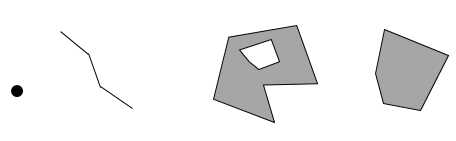
\includegraphics[scale=0.5]{figure1.png}
	\caption{Three basic spatial representations: points, lines, areas}
	\label{fig:figure1}
\end{figure}

Spatial objects relate to each other can be described by the form of partitions or networks as shown in Figure 2.2 below. 

\begin{figure}[h!]
	\centering
	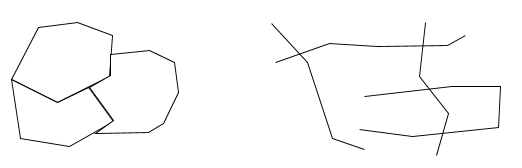
\includegraphics[scale=0.7]{figure2.png}
	\caption{Partitions and networks}
	\label{fig:figure2}
\end{figure}

A partition can be described by a group of separate region. The liaison between the regions is the regions’ equally boundary. For example, the partition can be used to represent a thematic map. A network can be illustrated by the graph that are connected in a field where each object point considered as nodes and lines as the geometric shapes of the edges. This network forms can be used to represent roads, rivers, public transportation, or electricity cable lines \cite{guting1994introduction}.


\section{Routing System}
Routing System is a system that provides driving directions or routes that can be taken by a moving object in order to reach a location of the destination. This system is often referred to the navigation system. Modern navigation systems now have integrated between the position of the object, sensors, computing, and communications between the hardware and software to support the facilities in humans, vehicles, and other moving objects. In addition, modern navigation systems also consider the geographical location coordinates distance accuracy, speed, and altitude of the moving object. The navigation system is widely used in outdoor data. But along with the times, this system is also applied to the indoor data.

\subsection{Outdoor Routing}
Outdoor routing technology is now highly developed. Figure 2.3 describes the flow of information on outdoor navigation systems.

\begin{figure}[h!]
	\centering
	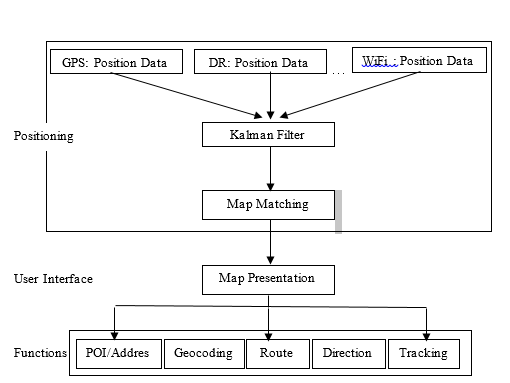
\includegraphics[scale=0.7]{figure3.png}
	\caption{The information flow on outdoor navigation systems \cite{karimi2011universal}}
	\label{fig:figure3}
\end{figure}

From Figure \ref{fig:figure3}, the user's position is determined by: (a) obtaining position data through geo-positioning sensor and (b) applying the map matching algorithm using position data obtained. These steps are general steps to improve the accuracy, availability, and reliability of outdoor navigation system by using more than one geo-positioning sensor in which each of the position data can be filtered using Kalman filter to find the best position estimation. Furthermore, the position data that has been filtered out will be inserted to the map matching algorithm that uses a database map for traveling the area, which contains spatial and non-spatial to find: (a) roads / pavements where users are located and (b) the location right of user in the segment.

When the user's location is known, the locations will be marked in the map and displayed to the user. At this stage, the system is currently tracking, and users have the option to search for POIs or a request for an optimal route between the pair of addresses. The system uses a search using the shortest or fastest route criteria \cite{karimi2011universal}. Figure \ref{fig:figure4} is an example of outdoor routing system implementation.

\begin{figure}[h!]
	\centering
	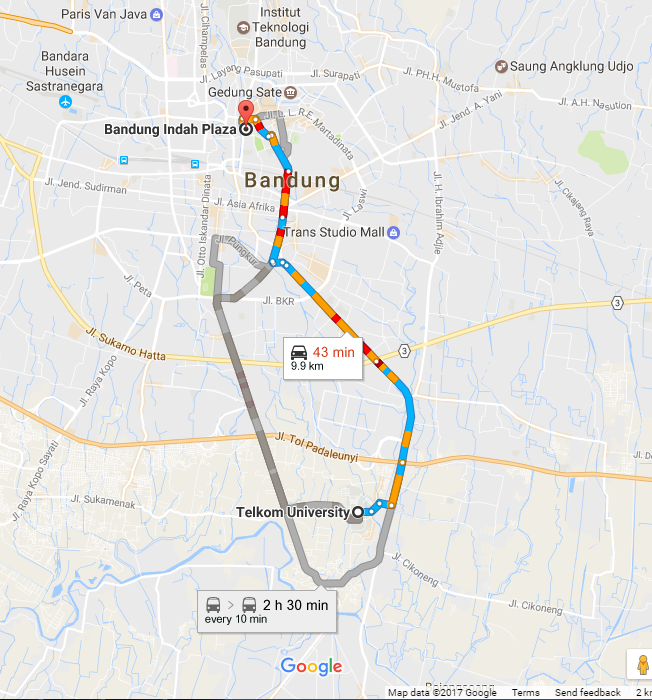
\includegraphics[scale=0.4]{figure4a.png}
	\caption{Examples of outdoor routing implementation}
	\label{fig:figure4}
\end{figure}

\subsection{Indoor Routing}
Indoor routing system is a routing system implementation in the building. By using spatial data, each space can be accurately identified. There are various kinds of elements in indoor spaces such as rooms, doors, corridors, floors, stairs, elevators, and the road connection between buildings. Indoor spaces are represented by undirected graph with nodes and edges. The concept of modeling the indoor spaces can be summarized in Table \ref{indoor-concept-table}.

\begin{table}[h!]
	\centering
	\caption{The concept of indoor spaces modeling \cite{alamri2014adjacency}} %\ref{fig:figure9}}
	\label{indoor-concept-table}
	\begin{tabular}{|l|l|l}
		\cline{1-2}
		\textbf{Domain Concept} & \textbf{Modeling Concept}   &  \\ \cline{1-2}
		Room		&	A cell &  \\ \cline{1-2}
		Door		&	An edge  &  \\ \cline{1-2}
		Corridor	&	One or more cells with one or more edges &  \\ \cline{1-2}
		Stair		&	One or more cells with one or more edges &  \\ \cline{1-2}
		Elevator	&	One cell with several edges &  \\ \cline{1-2}
		Pathway		&	One or more cells with several edges &  \\ \cline{1-2}
	\end{tabular}
\end{table}

As an illustration, Figure \ref{fig:figure5} is a graph modeling the indoor spaces delineated by one level.

\begin{figure}[h!]
	\centering
	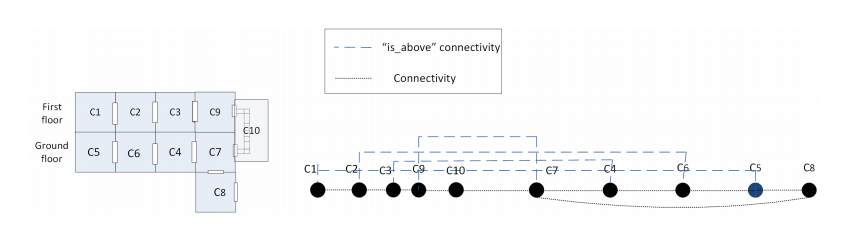
\includegraphics[scale=0.6]{figure5a.png}
	\caption{Modeling indoor spaces with a graph of the level \cite{alamri2014adjacency}}
	\label{fig:figure5}
\end{figure}

From the illustration, it can be seen that C10, C9, C8, C7, C4, C6, C5, C3, C2 and C1 are connected where C10 is the ladder that connects the ground floor and the first floor. Given this concept, it can be concluded that:
\begin{enumerate}
	\item An indoor space is a connected undirected graph (Cells, Edges), where Cells = {C1, C2, ..., Cn} is a set of cells, and Edges = {E1, E2, . . . , Em} is set of edges, each of which is a set of two cells, that is, each edge connects two distinct cells. 
	\item (Adjacent Nodes) Let G = (N,C) be a graph, and two Nodes n1,n2 $\in$ N of G are adjacent if: $\exists$ n1,n2 are connected.
	\item (Multidimensional Connectivity Graph) Given a set of cells Ci , Cj , Cf , Cl in the ground floor and a set of cells Cx, Cy,Cr, Ct the multidimensional connectivity graph refers to the multiple edges that connect the single floor cells and the above cells in the multi-floor space \cite{alamri2014adjacency}.
\end{enumerate}	 

\section{Shortest Path Algorithms}
There are several algorithms that the accuration and time complexity have been tested to calculate the shortest distance between nodes on a graph, like Dijkstra's and A* algorithms.
\subsection{Dijkstra's Algorithm}
For each vertex within a graph we assign a label that determines the minimal length from the starting point $s$ to other vertices $v$ of the graph. In a computer we can do it by declaring an array $d[]$. The algorithm works sequentially, and in each step it tries to decrease the value of the label of the vertices. The algorithm stops when all vertices have been visited. The label at the starting point $s$ is equal to zero $(d[s] = 0)$; however, labels in other vertices $v$ are equal to infinity $(d[v] =\infty)$, which means that the length from the starting point $s$ to other vertices is unknown. In a computer we can just use a very big number in order to represent infinity. In addition, for each vertex $v$ we have to identify whether it has been visited or not. In order to do that, we declare an array of Boolean type called $u[v]$, where initially, all vertices are assigned as unvisited $(u[v] = false)$. The Dijkstra’s algorithm consists of $n$ iterations. If all vertices have been visited, then the algorithm finishes. Otherwise, from the list of unvisited vertices we have to choose the vertex which has the minimum (smallest) value at its label (At the beginning, we will choose a starting point $s$). After that, we will consider all neighbors of this vertex (Neighbors of a vertex are those vertices that have common edges with the initial vertex). For each unvisited neighbor we will consider a new length, which is equal to the sum of the label’s value at the initial vertex $v (d[v])$ and the length of edge $l$ that connects them. If the resulting value is less than the value at the label, then we have to change the value in that label with the newly obtained value\cite{magzhan2013review}.
\begin{equation}\label{finding-minimum-neighbour-in-dijkstra}
	d [ neighbors ] = min ( d [ neighbors ] , d[ v ] + l )
\end{equation}

After considering all of the neighbors, we will assign the initial vertex as visited $(u[v] = true)$. After repeating this step $n$ times, all vertices of the graph will be visited and the algorithm finishes or terminates. The vertices that are not connected with the starting point will remain by being assigned to infinity. In order to restore the shortest path from the starting point to other vertices, we need to identify array $p []$, where for each vertex, where $v \neq s$, we will store the number of vertex $p[v]$, which penultimate vertices in the shortest path. In other words, a complete path from $s$ to $v$ is equal to the following statement.

\begin{equation}\label{finding-path-in-dijkstra}
P = ( s , … , p [ p [ p [ v ] ] ] , p [ p [ v ] ] , p [ v ] , v )	
\end{equation}

Figure \ref{fig:figure6} is the pseudocode of Dijkstra's algorithm.

\begin{figure}[h!]
	\centering
	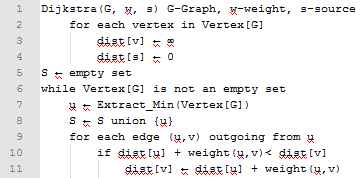
\includegraphics[scale=1]{figure6.png}
	\caption{Dijkstra's algorithm pseudocode}
	\label{fig:figure6}
\end{figure}

\subsection{Floyd-Warshall Algorithm}
Figure \ref{fig:figure7} is the pseudocode of Floyd-Warshall algorithm. Consider the graph $G$, where vertices were numbered from 1 to $n$. The notation dijk means the shortest path from $i$ to $j$, which also passes through vertex $k$. Obviously if there is exists edge between vertices $i$ and $j$ it will be equal to $d_{ij0}$, otherwise it can assigned as infinity. However, for other values of dijk there can be two choices: (1) If the shortest path from $i$ to $j$ does not pass through the vertex $k$ then value of $d_{ijk}$ will be equal to $d_{ijk- 1}$. (2) If the shortest path from $i$ to $j$ passes through the vertex $k$ then first it goes from $i$ to $k$, after that goes from $k$ to $j$. In this case the value of $d_{ijk}$ will be equal to $d_{ikk-1} + d_{kjk-1}$. And in order to determine the shortest path we just need to find the minimum of these two statements:


\begin{equation}\label{length-between-i-j}
	d_{ij0} = the \; length \; of \; edge \; between \; vertices \; i \; and \; j
\end{equation}

\begin{equation}\label{length-between-i-j}
	d_{ijk} = min (d_{ijk-1}, d_{ikk-1} + d_{kjk-1})	
\end{equation}

\begin{figure}[h!]
	\centering
	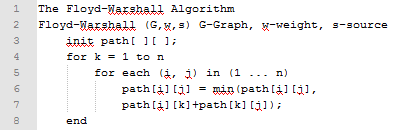
\includegraphics[scale=1]{figure7.png}
	\caption{Floyd-Warshall algorithm pseudocode}
	\label{fig:figure7}
\end{figure}
\vspace{40mm}
\subsection{Bellman-Ford Algorithm}
In comparison to Dijkstra’s algorithm, the Bellman-Ford algorithm admits or acknowledges the edges with negative weights. That is why, a graph can contain cycles of negative weights, which will generate numerous number of paths from the starting point to the final destination, where each cycle will minimize the length of the shortest path. Taking into consideration this fact, let’s assume that our graph does not contain cycles with negative weights. The array $d[]$ will store the minimal length from the starting point $s$ to other vertices. The algorithm consists of several phases, where in each phase it needs to minimize the value of all edges by replacing $d[b]$ to following statement $d[a] + c; a$ and $b$ are vertices of the graph, and $c$ is the corresponding edge that connects them. And in order to calculate the length of all shortest paths in a graph it requires $n – 1$ phases, but for those vertices of a graph that are unreachable, the value of elements of the array will remain by being assigned to infinity \cite{magzhan2013review}.

Figure 2.9 is the pseudocode of Bellman-Ford algorithm.
 
\begin{figure}[h!]
	\centering
	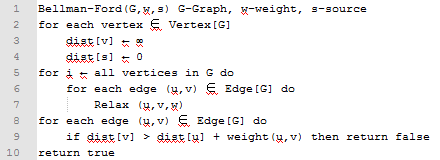
\includegraphics[scale=1]{figure8.png}
	\caption{Bellman-Ford algorithm pseudocode}
	\label{fig:figure8}
\end{figure}

\subsection{A* Algorithm}
The A* (called as ‘A-star’) (Cvetanovic and Nofsinger 1990) is like other graph searching algorithms in that it can potentially search a huge area of the map. It’s like Dijkstra’s algorithm in that it can be used to find a shortest path. It’s like breadth first search (BFS) in that it can use a heuristic to guide itself. In the simple case, it is as fast as BFS. Since in the worst case breadth-first search has to consider all paths to all possible nodes the time complexity of breadth-first search is increased depending on the number of nodes and edges in the graph \cite{sathyaraj2008multiple}.

This heuristic search ranks each node by an estimate of the best route that goes through that node. The typical formula is expressed as:

\begin{equation}\label{A-star-heuristic}
f(n) = g(n) + h(n)	
\end{equation}

where $f(n)$ is the score assigned to node $n$, this is the estimate of the best solution that goes through $n, g(n)$ is the actual cheapest cost of arriving at from the start node to $n$ and $h(n)$ is the heuristic estimate of the cost to the goal from $n$. Figure \ref{fig:figure9} is the pseudocode of A* algorithm.

\begin{figure}[h!]
	\centering
	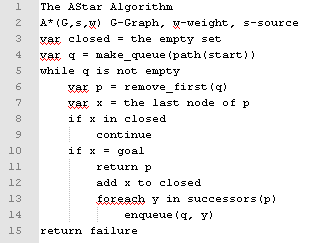
\includegraphics[scale=1]{figure9.png}
	\caption{A* algorithm pseudocode}
	\label{fig:figure9}
\end{figure}

\section{Three Dimensional Spaces}
Look at the example on Figure \ref{fig:figure10}. That is the picture of how the three dimensional spaces could be implement in representing the buildings. As you can see here, a building could be not just in one level, but it also could be a multi-level building. In this final project, each nodes of rooms, stairs, corridors will have its own three dimnesional attribute. $x$ attribute is the longitude coordinate in decimal, $y$ attribute is the latitude coordinate also in decimal. and $z$ attribute is the heigh or floor level of the building wich is in ordinal form.

\begin{figure}[h!]
	\centering
	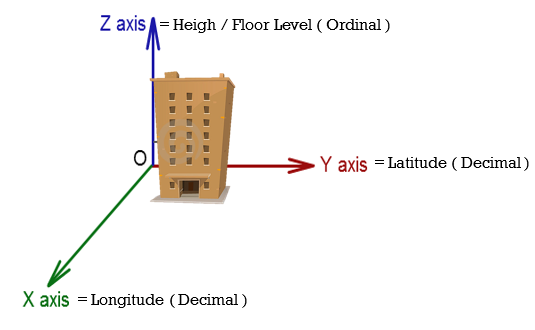
\includegraphics[scale=0.5]{figure10.png}
	\caption{Illustration of three dimensional spaces}
	\label{fig:figure10}
\end{figure}

\section{Distance between Two Points}
Measuring the distance between two points on a three dimensional space can be illustrated in Figure \ref{fig:figure11} below. If there is a power outlet in an area of a wall in a room and there is an electric iron on the table, how many minimum length of electric cable that needed to connect the iron to a power outlet? 

\begin{figure}[h!]
	\centering
	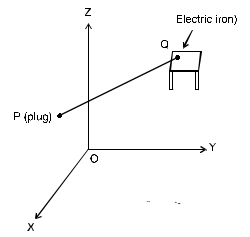
\includegraphics[scale=1]{figure11.png}
	\caption{Ilustration of distance between two points on a Three Dimensional Spaces}
	\label{fig:figure11}
\end{figure}

If the coordinates of the point $P$ is $(x_1, y_1, z_1)$ and point Q is $(x_2, y_2, z_2)$, then the distance between point $P$ and point $Q$ or $|PQ|$ can be determined by using the following formula:


\begin{equation}\label{distance-between-2-points}
|PQ|= \sqrt{(x_2 - x_1)^2 + (y_2 - y_1)^2 + (z_2 - z_1)^2}
\end{equation}

Thus, it can be seen that the general equation of distance point $P (x, y, z)$ to the center point $O (0,0,0)$ will be as follows:

\begin{equation}\label{A-star-heuristic}
|PQ|= \sqrt{(x_2 - 0)^2 + (y_2 - 0)^2 + (z_2 - 0)^2}
\end{equation}

\begin{equation}\label{A-star-heuristic}
|PQ|= \sqrt{(x_2)^2 + (y_2)^2 + (z_2)^2}
\end{equation}

In other case, such as the distance between a room in the first floor and the one in the third floor of a bilding, we can’t just use that formula to measure the distance. There is a route that we have to consider. Figure \ref{fig:figure12} shows the route wich include rooms, corridors, and stairs of a building. To measure the distance between room R1 and room R2, we have to measure the exact length of the route.

\begin{figure}[h!]
	\centering
	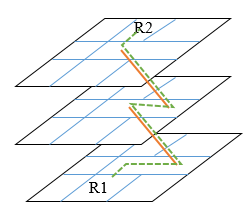
\includegraphics[scale=1]{figure12.png}
	\caption{Ilustration of distance between two rooms}
	\label{fig:figure12}
\end{figure}
\subsection{Spatial Data Distance Calculation using Haversine Formula}
The Haversine formula is an equation important in navigation, giving great-circle distances between two points on a sphere from their longitudes and latitudes. These names follow from the fact that they are customarily written in terms of the haversine function, given by $haversin (\theta) = sin^2
(\theta/2)$. The haversine formula is used to calculate the distance between two points on the Earth’s surface specified in longitude and latitude \cite{chopde2013landmark}.

\begin{equation}\label{A-star-heuristic}
d=2r sin^-1 ( \sqrt{sin^2 (\dfrac{\phi_2 - \phi_1}{2})}+cos(\phi_1)cos(\phi_2) sin^2(\dfrac{\psi_2-\psi_1}{2}))
\end{equation}

$d$ is the distance between two points with longitude and latitude $(\psi,\theta)$ and $r$ is the radius of the Earth.

\section{Summary}
This chapter is about the references that will be used in this final project. The theories and the algorithm will be implemented in building the Indoor Routing System.
%
\chapter{System Methodology and Design}
\section{General Description}
As the product of this final project, an application named TELUR IRIS (Telkom University Indoor Routing System) was made. This application is used for finding the shortest path between two rooms of Telkom University. Although, as declared in scope section of Chapter I, this application still use the data of D, E, and F Buildengs only. This application will show the user clearly about how the nodes of the graph represent the buildings by showing the nodes based on its three dimensional attribute. Several kinds of shortest path algorithm will be implemented and will be analyzed to get algorithm wich will give the best prformance that match this case.
  
\section{System Design}

\subsection{The Data Structure}
Dataset that used in this final project is the spatial data of Faculty of Informatics Telkom University, Bandung that include D, E, and F buildings. Figure \ref{fig:figure13} is the table relation of the dataset used in the TELUR IRIS Application. We need the data of buildings, rooms, corridors, stairs, and also Segments wich will be the relation or edges in the graph. For rooms, corridors, and stairs will have an attribute Building\textunderscore{ID} as a foreign key that reference to Building\textunderscore{ID} as the primary key of buildings. With this way, we know that each of rooms, corridors, and stairs is belongs to one of the buildings. However, for the corridor nodes that are outside the buildings, the Building\textunderscore{ID} attribute will be set as null value. Segments table has source and destination attribute that actually filled with the nodes ID in graph. 

\vspace{60mm}

\begin{figure}[h!]
	\centering
	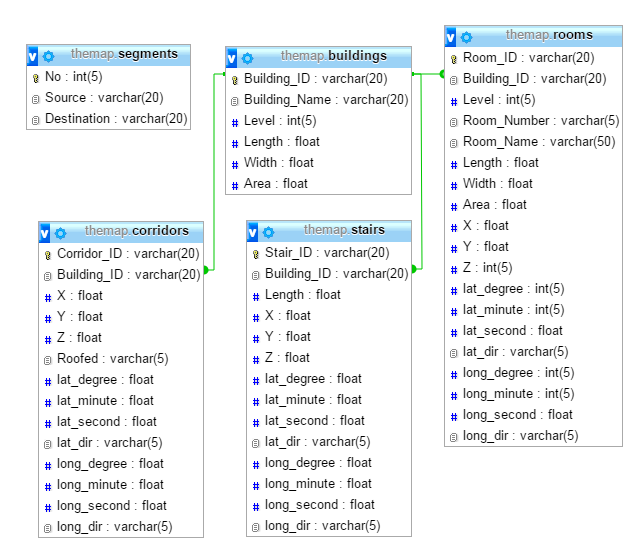
\includegraphics[scale=0.9]{figure13.png}
	\caption{Relational table of dataset}
	\label{fig:figure13}
\end{figure}

\vspace{60mm}

\subsection{System Flow}
The main process of this application can be modeled with the flow chart below.

\begin{figure}[h!]
	\centering
	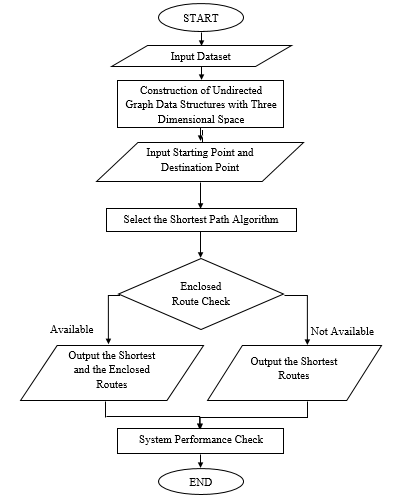
\includegraphics[scale=1.4]{figure14.png}
	\caption{System Flow Chart}
	\label{fig:figure14}
\end{figure}

\subsubsection{Construction of undirected Graph Data Structures with Three Dimensional Space}
At this stage, the construction of undirected graph data structure using three dimensional space representation of the existing data sets. Unlike the indoor routing data representation that already described in Chapter 2, this will represent multi-floor building in three dimensions based on the location of the coordinates x, y, and z coordinates of altitude. This final project use the study case of D, E, and F buildings of School of Computing in Telkom University, Bandung, Indonesia. Figure \ref{fig:figure19a} shows the area of Telokm University captured from Google Earth Application. The red rectanges are the D, E, and F buildings. Figure \ref{fig:figure19b}shows the zoomed in figure of D, E, and F buildings with the 2D graph modeling overlayed it. This is a way to get the longitude and latitude coordinates. 

\begin{figure}[h!]
	\centering
	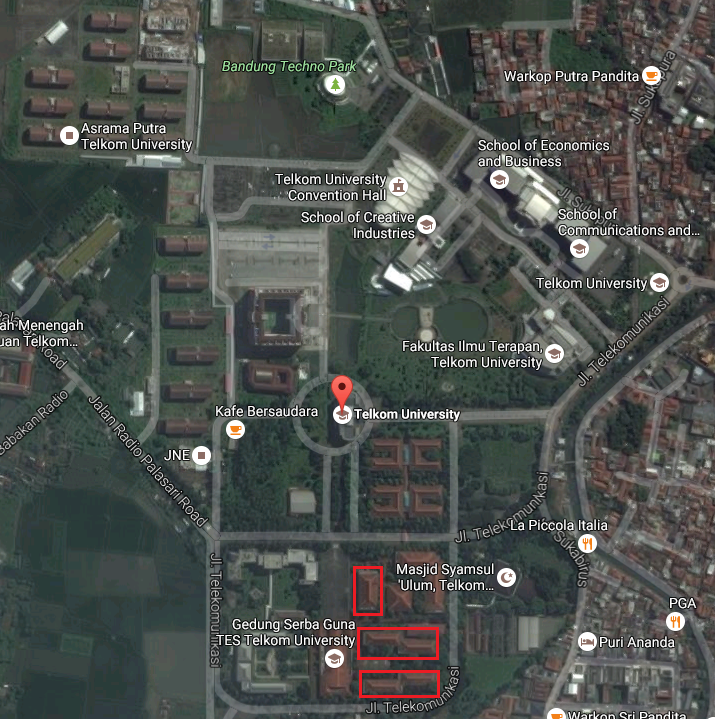
\includegraphics[scale=0.7]{figure19a.png}
	\caption{Telkom University area}
	\label{fig:figure19a}
\end{figure}

\begin{figure}[h!]
	\centering
	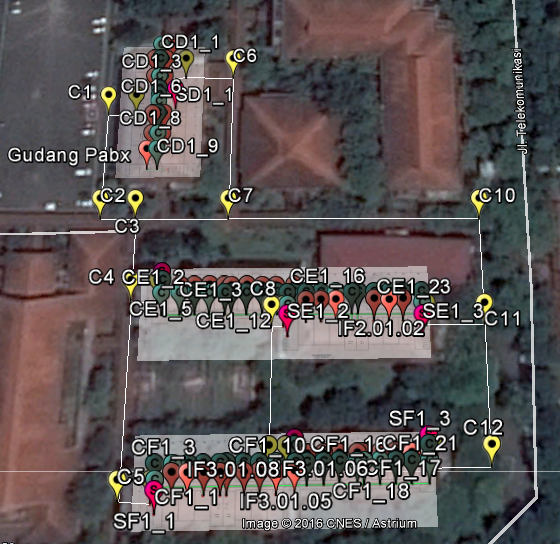
\includegraphics[scale=1]{figure19b.png}
	\caption{Telkom University area}
	\label{fig:figure19b}
\end{figure}



In the next step, the 3D modelling can be implemented in the system. This system show the 3D model as 2D model like shown in Figure \ref{fig:figure18} because a building is actually an overlayed multi-objects. To show the 3D modelling, coordinate shifting method could be implemented. Coordinate shifting method will move the x and y coordinate of the nodes so it would not be overlayed anymore. Illustration of Three Dimensional Spaces model can be seen in Figure \ref{fig:figure15}. red nodes mean the first level, green nodes mean the second floor, and blue ones mean the third floor.

\begin{figure}[h!]
	\centering
	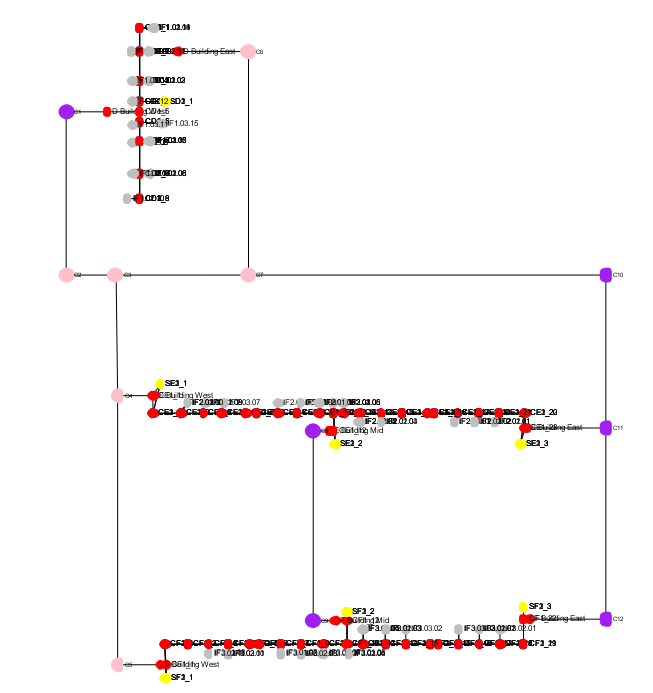
\includegraphics[scale=0.5]{figure18.PNG}
	\caption{2D system's graph modeling}
	\label{fig:figure18}
\end{figure}

\begin{figure}[h!]
	\centering
	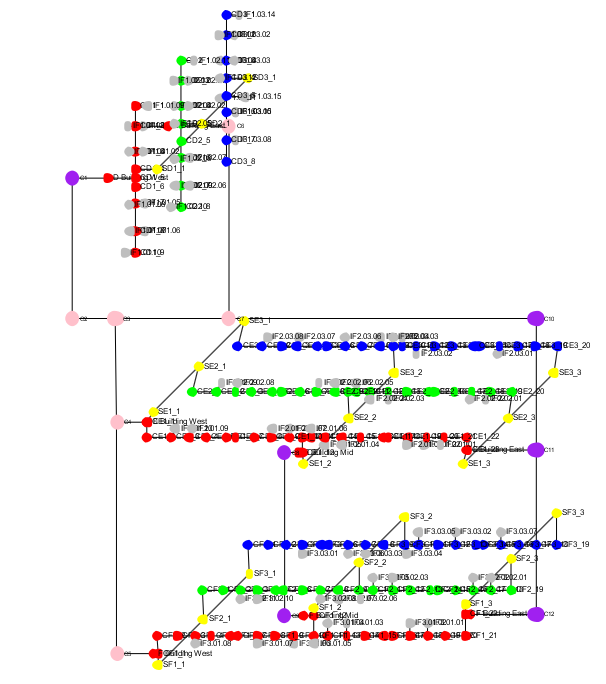
\includegraphics[scale=0.5]{figure15.PNG}
	\caption{3D system's graph modeling}
	\label{fig:figure15}
\end{figure}

\vspace{10mm}
\subsubsection{Finding the Shortest Path}
At this stage, shortest path algorithms will be implemented. There are Dijkstra's, Bellman-Ford, Floyd-Warshall, and A* algorithms that we could try to give the result of the shortest path. After the user choose one of the algorithms, shortest path searching will be done twice. The first search is using the full part of graph to show the shortest path weather it is open or close path. The second search will be eliminate nodes wich are the open space, so it will return a closed path.

By default, the system will show the close space path like the one shown in Figure \ref{fig:figure16}. But, by clicking the shortest path text area, it could easily change the view to the shortest path like shown in Figure \ref{fig:figure17}.

\begin{figure}[h!]
	\centering
	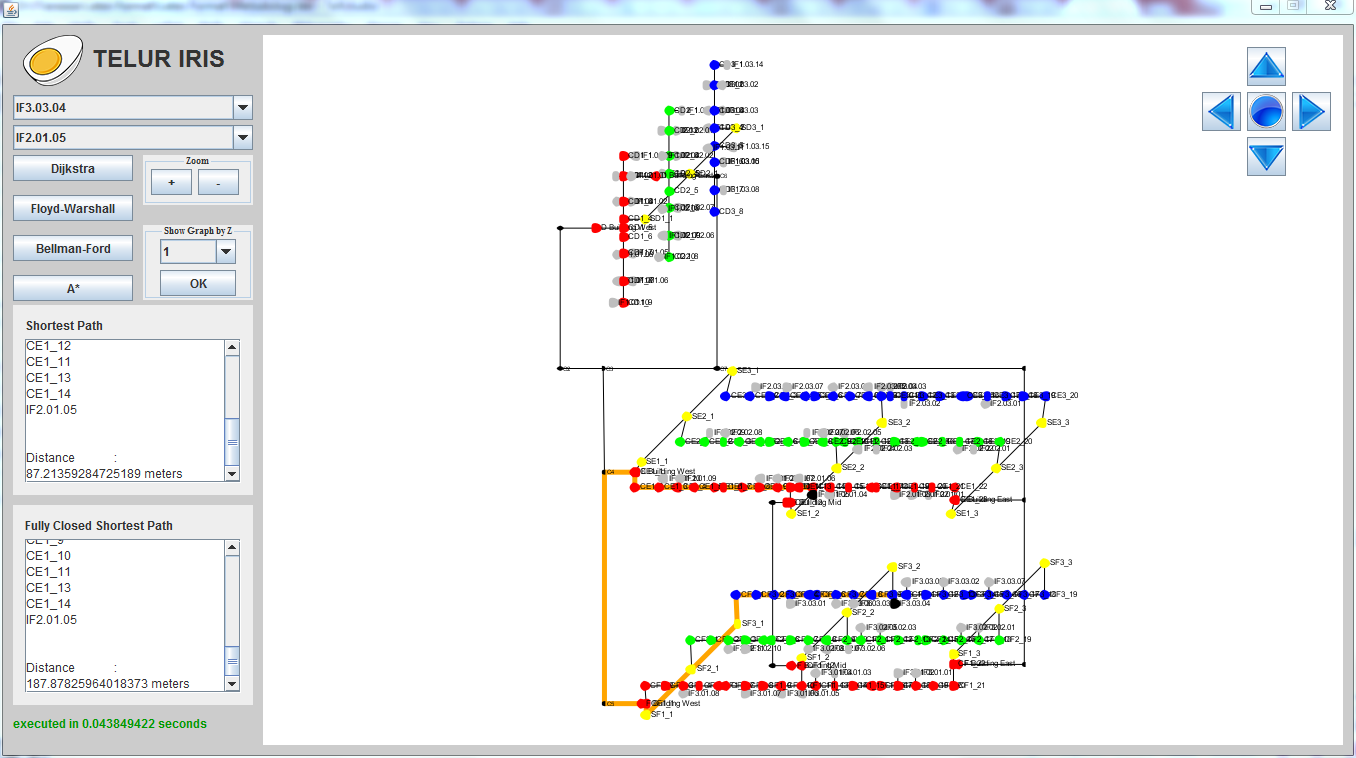
\includegraphics[scale=0.4]{figure16.PNG}
	\caption{The close space shortest path}
	\label{fig:figure16}
\end{figure}

\begin{figure}[h!]
	\centering
	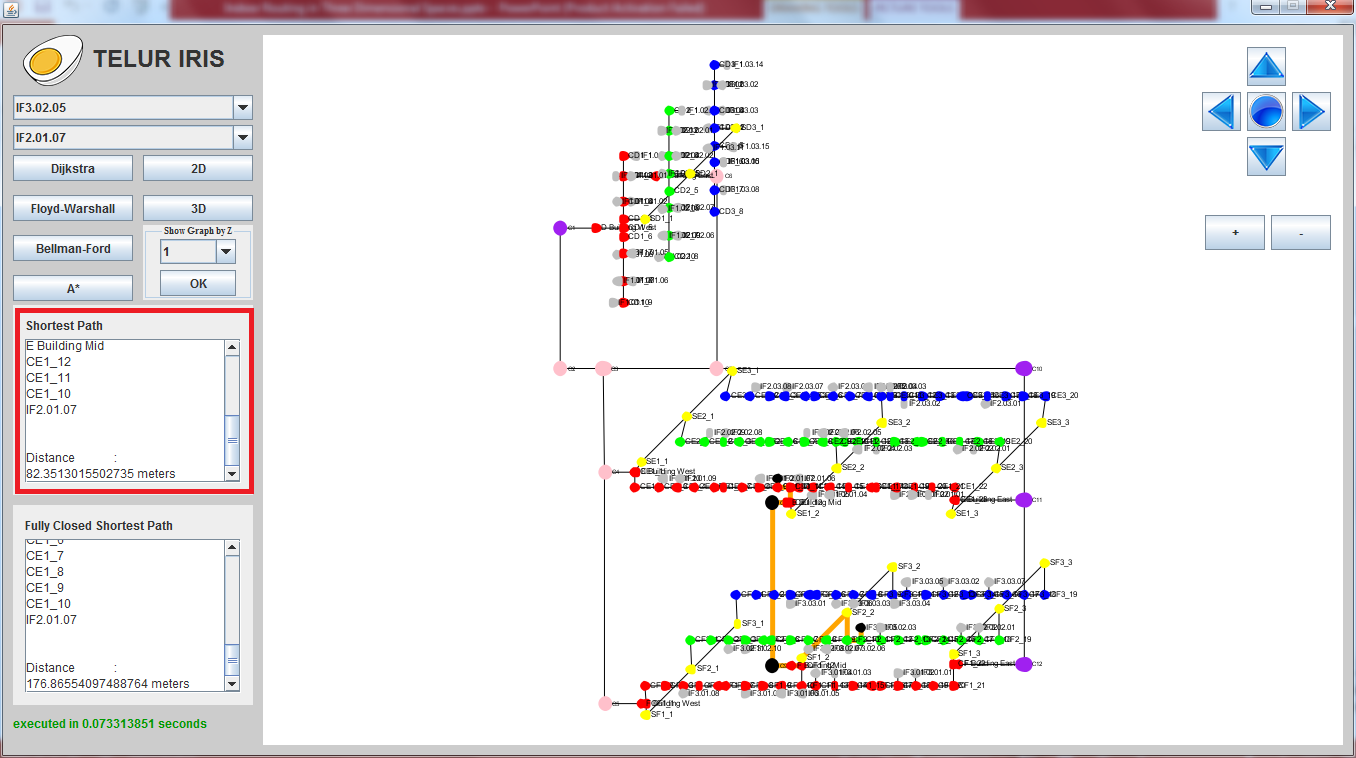
\includegraphics[scale=0.4]{figure17.PNG}
	\caption{The shortest path}
	\label{fig:figure17}
\end{figure}

\vspace{60mm}
\subsubsection{System Performance Check}
After the algorithm return the shortest paths, time execution will be measured at this stage.

\section{System Requirements Specification}
In this final project, the hardware and software that will support routing indoor systems to be built and work properly are:

\begin{enumerate}
	\item Hardware Specification\\
		Here is the following hardware specifications used in this final project.\\
		Model 	: Intel® Core™ i7-3770 CPU\\
		Prosesor	: 3.40 GHz Intel Core i7\\
		RAM	: 4 GB\\
		OS		: Windows 7 Professional 64 bit

	\item Software Specification\\
Here is the following software specifications used in this final project.\\
Application	:
\begin{itemize}
	\item Java Netbeans IDE 8.0.2
	\item JDK 1.8
	\item MySQL
\end{itemize}
\end{enumerate}

\section{Summary}
This chapter is about the plan of how to construct the Indoor Routing System using three dimensional spaces data structure. It also axplain the detail of the system flow and the system requirements.
%
\chapter{Testing and Analysis}
\section{System Testing}
In this chapter, will be explain about testing and analysis that used in this final project. The result of this testing and analyzing process will show how good the perfomance of the system is. There are two aspects that will be the concern in this step, they are execution time and the correctness of the outputs.  

\subsection{Testing Objective}
Based on the system model in chapter 3, the shortest path algorithms will be implemented in Indoor Routing System using three dimensional data structure. And the objectives of this testing process are:
\begin{enumerate}
%	\item Knowing that the shortest path algorithms can be implemented in three dimensional graph data structure.
	\item To get the best system's performance by comparing the execution time between Dijkstra's, Bellman-Ford, Floyd-Warshall, and A* algorithms.
	\item To get the system's accuracy by comparing the distance as the result of TELUR IRIS system and  the distance in real life.
\end{enumerate}

\subsection{Testing Scenario}
The following statements are the scenario of testing process:

\begin{enumerate}
	\item \textbf{Testing of system's perfomance in execution time}. In this section, each of dijkstra's, bellman-ford, floyd-warshall, and A* will be tested five times to get the execution time. After that the average amount can be assumed as the exact execution time. this testing will be implemented in both open and close space wich is has different count of nodes and edges.
	
	\item \textbf{Testing of system's accuracy}. In this section, comparison between the distance as the result of TELUR IRIS system and  the distance in real life will be calculated. For each scenario, there will be three samples of calculation result.
	
	The scenario of this test will be devided into 4, those are:
	\begin{itemize}
		\item Distance calculation between two rooms that have same Building\textunderscore{ID} and same $z$ attribute.
		\item Distance calculation between two rooms that have same Building\textunderscore{ID} but different $z$ attribute.
		\item Distance calculation between two rooms that have different Building\textunderscore{ID} but same $z$ attribute.
		\item Distance calculation between two rooms that have different Building\textunderscore{ID} and different $z$ attribute.
	\end{itemize}
	
\end{enumerate}

\section{Testing Result}

\subsection{Time Execution Comparison}
Here are the result of time execution testing. For the testing sample, the shortest path between node IF1.01.01 to node IF3.03.07 were choosen as a sample. This test implemented Dijkstra, Floyd-Warshall, Bellman-Ford, and A* Algorithms to search that shortest path. The testing do the searching process five times for each algorithms and it took the average value of the execution times as the result. All the time values are in seconds. 
\\\\
\textbf{The output of five times Dijkstra's Algorithm running:}\\
*****dijkstra algorithm node IF1.01.01 to IF3.03.07*****\\
graph.getNodeCount() = 272\\
execution time dijkstra : 0.176570559\\
*****dijkstra algorithm node IF1.01.01 to IF3.03.07*****\\
graph.getNodeCount() = 266\\
execution time dijkstra\textunderscore{close} : 0.059495901\\
executed in 0.23606646 seconds\\
\\
*****dijkstra algorithm node IF1.01.01 to IF3.03.07*****\\
graph.getNodeCount() = 272\\
execution time dijkstra : 0.059805929\\
*****dijkstra algorithm node IF1.01.01 to IF3.03.07*****\\
graph.getNodeCount() = 266\\
execution time dijkstra\textunderscore{close} : 0.030269795\\
executed in 0.090075724 seconds\\
\\
*****dijkstra algorithm node IF1.01.01 to IF3.03.07*****\\
graph.getNodeCount() = 272\\
execution time dijkstra : 0.048037625\\
*****dijkstra algorithm node IF1.01.01 to IF3.03.07*****\\
graph.getNodeCount() = 266\\
execution time dijkstra\textunderscore{close} : 0.035783754\\
executed in 0.083821379 seconds\\
\\
*****dijkstra algorithm node IF1.01.01 to IF3.03.07*****\\
graph.getNodeCount() = 272\\
execution time dijkstra : 0.04465599\\
*****dijkstra algorithm node IF1.01.01 to IF3.03.07*****\\
graph.getNodeCount() = 266\\
execution time dijkstra\textunderscore{close} : 0.030038336\\
executed in 0.074694326 seconds\\
\\
*****dijkstra algorithm node IF1.01.01 to IF3.03.07*****\\
graph.getNodeCount() = 272\\
execution time dijkstra : 0.06649877\\
*****dijkstra algorithm node IF1.01.01 to IF3.03.07*****\\
graph.getNodeCount() = 266\\
execution time dijkstra\textunderscore{close} : 0.032153671\\
executed in 0.098652441 seconds\\
\\\\
\textbf{The output of five times Floyd-Warshall Algorithm running:}\\
*****Floyd-Warshal algorithm node IF1.01.01 to IF3.03.07*****\\
graph.getNodeCount() = 272\\
execution time fw : 0.280716078\\
*****Floyd-Warshal algorithm node IF1.01.01 to IF3.03.07*****\\
graph.getNodeCount() = 266\\
execution time fw\textunderscore{close} : 0.175645076\\
executed in 0.456361154 seconds\\
\\
*****Floyd-Warshal algorithm node IF1.01.01 to IF3.03.07*****\\
graph.getNodeCount() = 272\\
execution time fw : 0.262804205\\
*****Floyd-Warshal algorithm node IF1.01.01 to IF3.03.07*****\\
graph.getNodeCount() = 266\\
execution time fw\textunderscore{close} : 0.100703012\\
executed in 0.363507217 seconds\\
\\
*****Floyd-Warshal algorithm node IF1.01.01 to IF3.03.07*****\\
graph.getNodeCount() = 272\\
execution time fw : 0.295337272\\
*****Floyd-Warshal algorithm node IF1.01.01 to IF3.03.07*****\\
graph.getNodeCount() = 266\\
execution time fw\textunderscore{close} : 0.081183668\\
executed in 0.37652094 seconds\\
\\
*****Floyd-Warshal algorithm node IF1.01.01 to IF3.03.07*****\\
graph.getNodeCount() = 272\\
execution time fw : 0.283726813\\
*****Floyd-Warshal algorithm node IF1.01.01 to IF3.03.07*****\\
graph.getNodeCount() = 266\\
execution time fw\textunderscore{close} : 0.238191704\\
executed in 0.521918517 seconds\\
\\
*****Floyd-Warshal algorithm node IF1.01.01 to IF3.03.07*****\\
graph.getNodeCount() = 272\\
execution time fw : 0.282648442\\
*****Floyd-Warshal algorithm node IF1.01.01 to IF3.03.07*****\\
graph.getNodeCount() = 266\\
\\execution time fw\textunderscore{close} : 0.263365865
\\executed in 0.546014307 seconds
\\\\
\\\textbf{The output of five times Bellman-Ford Algorithm running:}
\\*****Bellman-Ford algorithm node IF1.01.01 to IF3.03.07*****
\\graph.getNodeCount() = 272
\\execution time bf : 0.337928182
\\*****Bellman-Ford algorithm node IF1.01.01 to IF3.03.07*****
\\graph.getNodeCount() = 266
\\execution time bf\textunderscore{close} : 0.188902291
\\executed in 0.526830473 seconds
\\
\\*****Bellman-Ford algorithm node IF1.01.01 to IF3.03.07*****
\\graph.getNodeCount() = 272
\\execution time bf : 0.221083213
\\*****Bellman-Ford algorithm node IF1.01.01 to IF3.03.07*****
\\graph.getNodeCount() = 266
\\execution time bf\textunderscore{close} : 0.234484116
\\executed in 0.455567329 seconds
\\
\\*****Bellman-Ford algorithm node IF1.01.01 to IF3.03.07*****
\\graph.getNodeCount() = 272
\\execution time bf : 0.29284962
\\*****Bellman-Ford algorithm node IF1.01.01 to IF3.03.07*****
\\graph.getNodeCount() = 266
\\execution time bf\textunderscore{close} : 0.240597956
\\executed in 0.533447576 seconds
\\
\\*****Bellman-Ford algorithm node IF1.01.01 to IF3.03.07*****
\\graph.getNodeCount() = 272
\\execution time bf : 0.273845218
\\*****Bellman-Ford algorithm node IF1.01.01 to IF3.03.07*****
\\graph.getNodeCount() = 266
\\execution time bf\textunderscore{close} : 0.246817972
\\executed in 0.52066319 seconds
\\
\\*****Bellman-Ford algorithm node IF1.01.01 to IF3.03.07*****
\\graph.getNodeCount() = 272
\\execution time bf : 0.28561423
\\*****Bellman-Ford algorithm node IF1.01.01 to IF3.03.07*****
\\graph.getNodeCount() = 266
\\execution time bf\textunderscore{close} : 0.236419664
\\executed in 0.522033894 seconds
\\\\
\\\textbf{The output of five times A* Algorithm running:}
\\*****A* algorithm node IF1.01.01 to IF3.03.07*****
\\graph.getNodeCount() = 272
\\execution time astar : 0.065852526
\\*****A* algorithm node IF1.01.01 to IF3.03.07*****
\\graph.getNodeCount() = 266
\\execution time astar\textunderscore{close} : 0.016076835
\\executed in 0.081929361 seconds
\\
\\*****A* algorithm node IF1.01.01 to IF3.03.07*****
\\graph.getNodeCount() = 272
\\execution time astar : 0.03272878
\\*****A* algorithm node IF1.01.01 to IF3.03.07*****
\\graph.getNodeCount() = 266
\\execution time astar\textunderscore{close} : 0.023422293
\\executed in 0.056151073 seconds
\\
\\*****A* algorithm node IF1.01.01 to IF3.03.07*****
\\graph.getNodeCount() = 272
\\execution time astar : 0.030558941
\\*****A* algorithm node IF1.01.01 to IF3.03.07*****
\\graph.getNodeCount() = 266
\\execution time astar\textunderscore{close} : 0.01713822
\\executed in 0.047697161 seconds
\\
\\*****A* algorithm node IF1.01.01 to IF3.03.07*****
\\graph.getNodeCount() = 272
\\execution time astar : 0.026007271
\\*****A* algorithm node IF1.01.01 to IF3.03.07*****
\\graph.getNodeCount() = 266
\\execution time astar\textunderscore{close} : 0.022123787
\\executed in 0.048131058 seconds
\\
\\*****A* algorithm node IF1.01.01 to IF3.03.07*****
\\graph.getNodeCount() = 272
\\execution time astar : 0.036428937
\\*****A* algorithm node IF1.01.01 to IF3.03.07*****
\\graph.getNodeCount() = 266
\\execution time astar\textunderscore{close} : 0.032021663
\\executed in 0.0684506 seconds
\\\\

The tables below shows the clearer comparison according to the console output of the system above. Table \ref{table:2} shows the comparison of the shortest path algorithms in showing the actual shortest path where all nodes (total 272 nodes) of the graph are included in the algorithm's calculation. Table \ref{table:3} shows the comparison of the shortest path algorithms in showing the shortest path in close space where nodes wich are the open space will not be calculated in shortest path algorithm (total 266 nodes).


% Please add the following required packages to your document preamble:
% \usepackage[table,xcdraw]{xcolor}
% If you use beamer only pass "xcolor=table" option, i.e. \documentclass[xcolor=table]{beamer}
\begin{table}[h!]
	\centering
	\caption{Shortest path execution time comparison for Whole Space}
	\label{table:2}
	\begin{tabular}{|c|l|l|l|l|}
		\hline
		\textbf{Itteration}                                            & \multicolumn{1}{c|}{\textbf{Dijkstra}} & \multicolumn{1}{c|}{\textbf{Floyd-Warshall}} & \multicolumn{1}{c|}{\textbf{Bellman-Ford}} & \multicolumn{1}{c|}{\textbf{A*}} \\ \hline
		1                                                              & 0.176570559                            & 0.280716078                                  & 0.337928182                                & 0.065852526                      \\ \hline
		2                                                              & 0.059805929                            & 0.262804205                                  & 0.221083213                                & 0.03272878                       \\ \hline
		3                                                              & 0.048037625                            & 0.295337272                                  & 0.29284962                                 & 0.030558941                      \\ \hline
		4                                                              & 0.04465599                             & 0.283726813                                  & 0.273845218                                & 0.026007271                      \\ \hline
		5                                                              & 0.06649877                             & 0.282648442                                  & 0.28561423                                 & 0.036428937                      \\ \hline
		\rowcolor[HTML]{9B9B9B} 
		\multicolumn{1}{|l|}{\cellcolor[HTML]{9B9B9B}\textbf{AVERAGE}} & 0.079113775                            & 0.281046562                                  & 0.282264093                                & 0.038315291                      \\ \hline
	\end{tabular}
\end{table}

% Please add the following required packages to your document preamble:
% \usepackage[table,xcdraw]{xcolor}
% If you use beamer only pass "xcolor=table" option, i.e. \documentclass[xcolor=table]{beamer}
\begin{table}[h!]
	\centering
	\caption{Shortest path execution time comparison for Close Space}
	\label{table:3}
	\begin{tabular}{|c|l|l|l|l|}
		\hline
		\textbf{Itteration}                                            & \multicolumn{1}{c|}{\textbf{Dijkstra}} & \multicolumn{1}{c|}{\textbf{Floyd-Warshall}} & \multicolumn{1}{c|}{\textbf{Bellman-Ford}} & \multicolumn{1}{c|}{\textbf{A*}} \\ \hline
		1                                                              & 0.059495901                            & 0.175645076                                  & 0.188902291                                & 0.016076835                      \\ \hline
		2                                                              & 0.030269795                            & 0.100703012                                  & 0.234484116                                & 0.023422293                      \\ \hline
		3                                                              & 0.035783754                            & 0.081183668                                  & 0.240597956                                & 0.01713822                       \\ \hline
		4                                                              & 0.030038336                            & 0.238191704                                  & 0.246817972                                & 0.022123787                      \\ \hline
		5                                                              & 0.032153671                            & 0.263365865                                  & 0.236419664                                & 0.032021663                      \\ \hline
		\rowcolor[HTML]{9B9B9B} 
		\multicolumn{1}{|l|}{\cellcolor[HTML]{9B9B9B}\textbf{AVERAGE}} & 0.037548291                            & 0.171817865                                  & 0.2294444                                  & 0.02215656                       \\ \hline
	\end{tabular}
\end{table}
\vspace{8mm}
And since the system will give both open and close space shortest paths, the comparison of system's time execution will be the total value of both situation. The value are shown in Table \ref{table:4}.

% Please add the following required packages to your document preamble:
% \usepackage[table,xcdraw]{xcolor}
% If you use beamer only pass "xcolor=table" option, i.e. \documentclass[xcolor=table]{beamer}
\begin{table}[h!]
	\centering
	\caption{System's execution time comparison}
	\label{table:4}
	\begin{tabular}{|c|l|l|l|l|}
		\hline
		\textbf{Itteration}                                            & \multicolumn{1}{c|}{\textbf{Dijkstra}} & \multicolumn{1}{c|}{\textbf{Floyd-Warshall}} & \multicolumn{1}{c|}{\textbf{Bellman-Ford}} & \multicolumn{1}{c|}{\textbf{A*}} \\ \hline
		1                                                              & 0.23606646                             & 0.456361154                                  & 0.526830473                                & 0.081929361                      \\ \hline
		2                                                              & 0.090075724                            & 0.363507217                                  & 0.455567329                                & 0.056151073                      \\ \hline
		3                                                              & 0.083821379                            & 0.37652094                                   & 0.533447576                                & 0.047697161                      \\ \hline
		4                                                              & 0.074694326                            & 0.521918517                                  & 0.52066319                                 & 0.048131058                      \\ \hline
		5                                                              & 0.098652441                            & 0.546014307                                  & 0.522033894                                & 0.0684506                        \\ \hline
		\rowcolor[HTML]{9B9B9B} 
		\multicolumn{1}{|l|}{\cellcolor[HTML]{9B9B9B}\textbf{AVERAGE}} & 0.116662066                            & 0.452864427                                  & 0.511708492                                & 0.02215656                       \\ \hline
	\end{tabular}
\end{table}

According to the data above, pictures below are the chart figures that show how far are the execution time deviation between each shortest path algorithms.

\begin{figure}[h!]
	\centering
	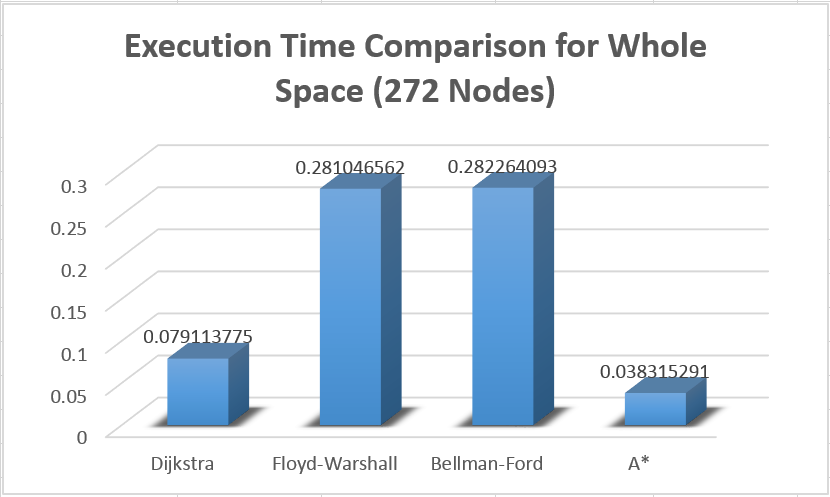
\includegraphics[scale=0.4]{graf1.PNG}
	\caption{Execution Time Comparison for Whole Space}
	\label{fig:graf1}
\end{figure}

\begin{figure}[h!]
	\centering
	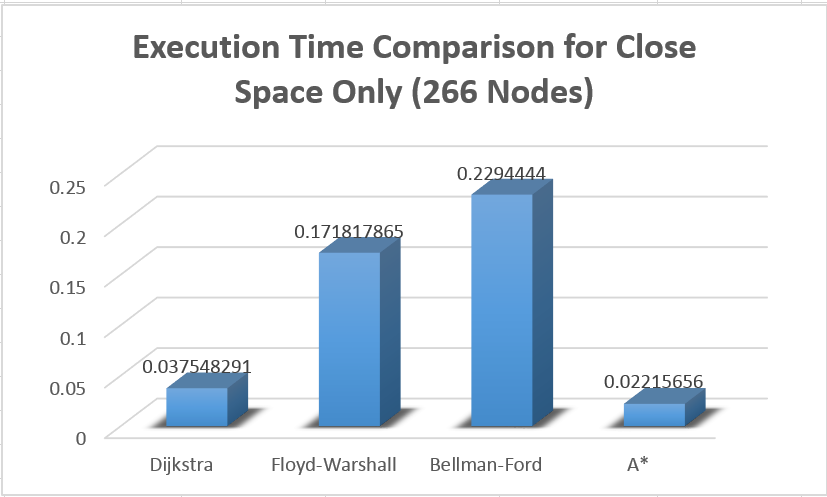
\includegraphics[scale=0.4]{graf2.PNG}
	\caption{Execution Time Comparison for Close Space Only}
	\label{fig:graf2}
\end{figure}

\begin{figure}[h!]
	\centering
	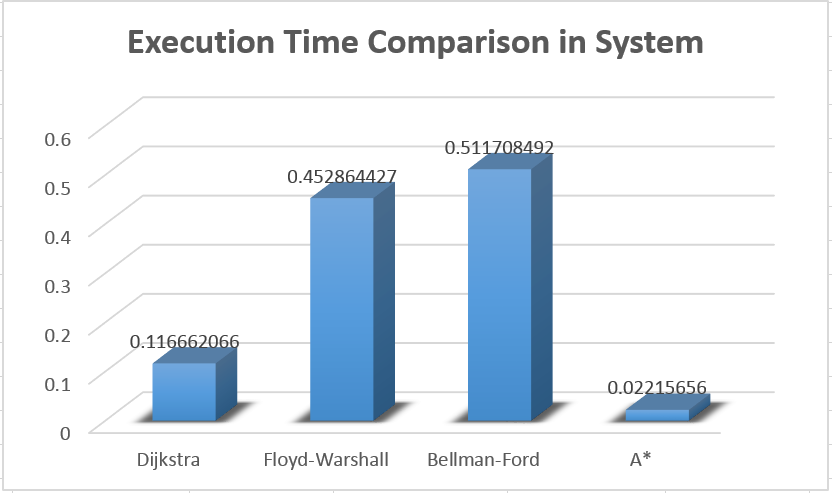
\includegraphics[scale=0.4]{graf3.PNG}
	\caption{Execution Time Comparison in System
	}
	\label{fig:graf3}
\end{figure}

\vspace{10mm}
As seen in the charts above, it could be concluded that A* Algorithm give the smallest execution time wich mean A* algorithm is the best algorithm to implement in this case besides Dijkstra, Floyd-Warshall, or Bellman-Ford algorithm. 
\vspace{60mm}
\subsection{Distance Calculation Comparison}
Here are the result of the system's accuracy testing. This testing will show the deviation between the result of system calculation and the real distance as shown in Table \ref{table:6}. All the distances are in meters.

% Please add the following required packages to your document preamble:
% \usepackage[table,xcdraw]{xcolor}
% If you use beamer only pass "xcolor=table" option, i.e. \documentclass[xcolor=table]{beamer}
\begin{table}[h!]
	\centering
	\caption{Distance deviation between system result and in the real life}
	\label{table:6}
	\begin{tabular}{|c|l|l|l|l|l|}
		\hline
		\rowcolor[HTML]{C0C0C0} 
		\textbf{No.} & \multicolumn{1}{c|}{\cellcolor[HTML]{C0C0C0}\textbf{Source}} & \multicolumn{1}{c|}{\cellcolor[HTML]{C0C0C0}\textbf{Destination}} & \multicolumn{1}{c|}{\cellcolor[HTML]{C0C0C0}\textbf{SPD\_S}} & \multicolumn{1}{c|}{\cellcolor[HTML]{C0C0C0}\textbf{SPD\_R}} & \multicolumn{1}{c|}{\cellcolor[HTML]{C0C0C0}\textbf{\begin{tabular}[c]{@{}c@{}}Deviation \\ ($ABS\left( SP\_S-SP\_R\right)$ )\end{tabular}}} \\ \hline
		1            & IF3.03.04                                                    & IF3.03.05                                                         & 8.661221996                                                  & 6                                                            & \cellcolor[HTML]{FFFC9E}2.661221996                                                                                        \\ \hline
		2            & IF3.02.05                                                    & IF3.02.01                                                         & 34.78388051                                                  & 34.7                                                         & \cellcolor[HTML]{FFFC9E}0.083880508                                                                                        \\ \hline
		3            & IF3.01.02                                                    & IF3.01.03                                                         & 21.56047226                                                  & 21.7                                                         & \cellcolor[HTML]{FFFC9E}0.139527743                                                                                        \\ \hline
		4            & IF3.03.03                                                    & IF3.02.05                                                         & 38.7783564                                                   & 34.1                                                         & \cellcolor[HTML]{FFFC9E}4.6783564                                                                                          \\ \hline
		5            & IF3.03.03                                                    & IF3.01.05                                                         & 41.18405404                                                  & 35.4                                                         & \cellcolor[HTML]{FFFC9E}5.784054043                                                                                        \\ \hline
		\rowcolor[HTML]{FFFFFF} 
		6            & IF2.01.10                                                    & IF2.02.09                                                         & 36.66114963                                                  & 31                                                           & 5.661149626                                                                                        \\ \hline
		7            & IF2.01.10                                                    & IF3.01.08                                                         & 102.1953267                                                  & 89.4                                                         & \cellcolor[HTML]{FFFC9E}12.79532672                                                                                        \\ \hline
	\end{tabular}
\end{table}

Figure \ref{fig:graf3} shows the fluctuation of the testing deviation result. From the chart, we can see that the daviation result is quiet fluctuate. This result means that this system has a deficiency in resuting the distance with average deviation velue is 4.543359576 meters.


\begin{figure}[h!]
	\centering
	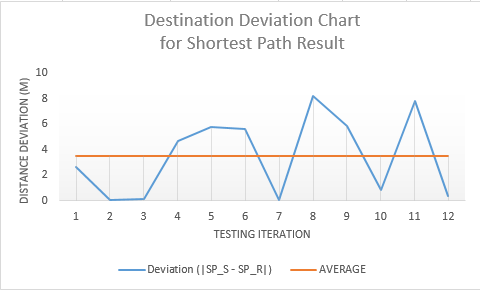
\includegraphics[scale=1]{graf4.PNG}
	\caption{Distance deviation testing result 
	}
	\label{fig:graf3}
\end{figure}

\section{Summary}

%
\chapter{Conclusions and Recommendations}
\section{Conclusions}
After the implementation, testing, and analyzing process have been done, it could be concluded that:
\begin{enumerate}
	\item Indoor Routing System could be implemented using three dimensional spaces.
	
	\item The most suitable Shortest Path Algorithm to the three dimensional spaces data between Dijkstra, Floyd-Warshall, Bellman-Ford, and A* Algorithms is A* Algorithm that give the smallest value of execution time.
	
	\item Floyd-Warshall and Bellman-Ford algorithms are not yet can be implemented in this case because Floyd–Warshall algorithm solves all pairs shortest distance, Bellman–Ford algorithm solves the single-source problem if edge weights may be negative, and both algorithms are not resulting the path but just the shortest distance value. Modification of these algorithms may could make it work.
	
	\item This System still lack of resulting the exact distance after it compared with the distance in real life. There are a few reason of this lackness such as the process in getting the nodes’ coordinate is still not accurate enough and for buildings that have a bit length of stairs to connect to the outter space, it assumed as one heigh level, so there will be a little bit difference between the calculation result and the measurement result. In this case, the calculation result could be called as an APPROXIMATE DISTANCE.
	
\end{enumerate}

\vspace{40mm}
\section{Future Work}
Since this final project have been done, there are a few recommendations to make this project better, those are:
\begin{enumerate}
	\item Add some more dataset until the whole area of Telkom University. After that, it could be published in college's website so this system could be used for everyone.
	\item Find another better way to get the exact longitude and latitude for the points. One of the examples is take a long walk from points to points and record the Longitude and Latitude coordinates.
	\item It would be better if the graph could be viewed with the 3D blueprints of the buildings. 
	\item Try to implement hub labeling algorithm to get the shortest path. 
	
\end{enumerate}

%
%\cleardoublepage
\addcontentsline{toc}{chapter}{Bibliography}

\bibliographystyle{acm} %harvard style
\bibliography{References}
%
%\pagebreak
%\cleardoublepage
\renewcommand\thesection{\Alph{section}}
\renewcommand\thesubsection{\thesection.\Alph{subsection}}
\addcontentsline{toc}{chapter}{Appendices}
\appendix
\chapter*{Appendices}

%\appendix
\section{The Database} \label{App:AppendixA}
% the \\ insures the section title is centered below the phrase: AppendixA
%Text of Appendix A is Here
\newcommand{\comm}[1]{}
\comm{
\begin{table}[h!]
	\centering
	\caption{Building Database}
	\label{my-label}
	\begin{tabular}{|l|l|l|l|l|l|l|}
		\hline
		\multicolumn{1}{|c|}{\textbf{No.}} & \multicolumn{1}{c|}{\textbf{Building ID}} & \multicolumn{1}{c|}{\textbf{Building Name}} & \multicolumn{1}{c|}{\textbf{Level}} & \multicolumn{1}{c|}{\textbf{Length}} & \multicolumn{1}{c|}{\textbf{Width}} & \multicolumn{1}{c|}{\textbf{Area}} \\ \hline
		1                                  & IF1                                       & Panambulai                                  & 3                                   & 0                                    & 0                                   & 0                                  \\ \hline
		2                                  & IF2                                       & Kultubai Utara                              & 3                                   & 88.8                                 & 0                                   & 0                                  \\ \hline
		3                                  & IF3                                       & Kultubai Selatan                            & 3                                   & 88.8                                 & 0                                   & 0                                  \\ \hline
	\end{tabular}
\end{table}

}

\begin{figure}[h!]
	\centering
	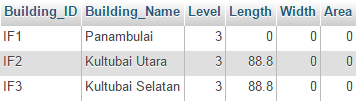
\includegraphics[scale=1]{DBbuilding.PNG}
	\caption{Example of building database (total 3 data)
	}
	\label{DBbuilding}
\end{figure}

\begin{figure}[h!]
	\centering
	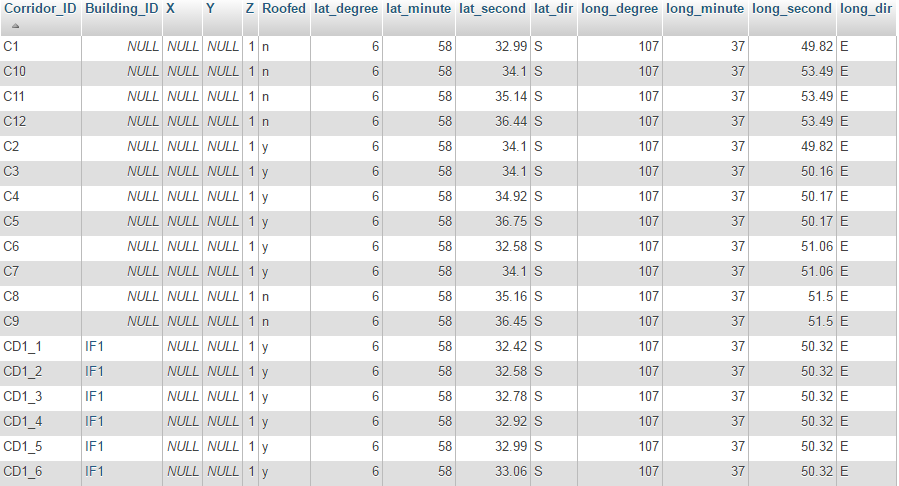
\includegraphics[scale=0.7]{DBcorridor.PNG}
	\caption{Example of corridor database (total 168 data)
	}
	\label{DBcorridor}
\end{figure}

\begin{figure}[h!]
	\centering
	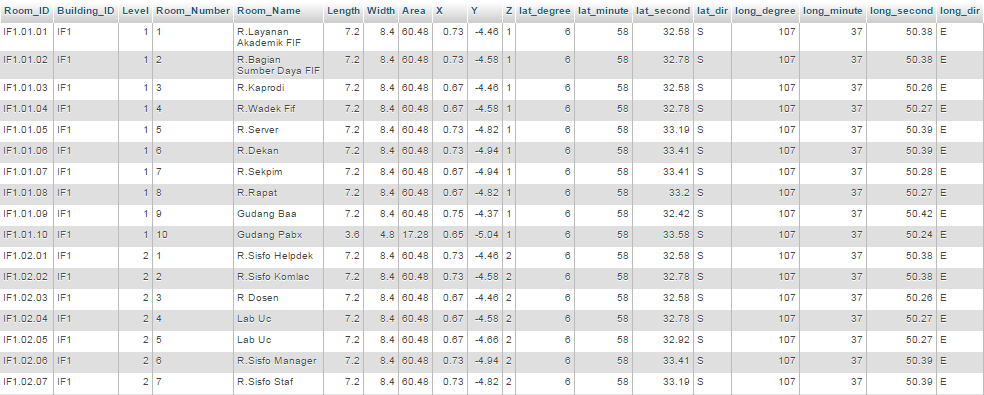
\includegraphics[scale=0.6]{DBroom.PNG}
	\caption{Example of room database (total 83 data)
	}
	\label{DBcorridor}
\end{figure}

\begin{figure}[h!]
	\centering
	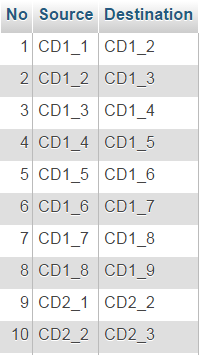
\includegraphics[scale=0.6]{DBsegment.PNG}
	\caption{Example of segment database (total 283 data)
	}
	\label{DBsegment}
\end{figure}

\begin{figure}[h!]
	\centering
	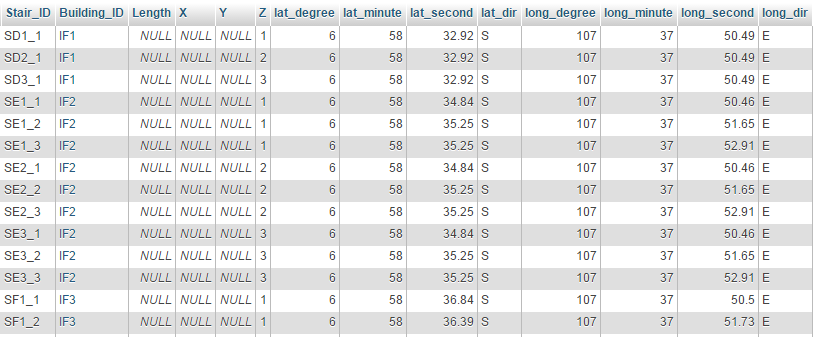
\includegraphics[scale=0.6]{DBstair.PNG}
	\caption{Example of stair database (total 21 data)
	}
	\label{DBstairt}
\end{figure}

\vspace{30mm}
\section{Floyd-Warshall Algorithm Testing}
% Please add the following required packages to your document preamble:
% \usepackage[table,xcdraw]{xcolor}
% If you use beamer only pass "xcolor=table" option, i.e. \documentclass[xcolor=table]{beamer}
\begin{table}[h!]
	\centering
	\caption{Floyd-Warshall Testing Iteration}
	\label{my-label}
	\begin{tabular}{|l|l|l|l|l|l|l|l|l|l|}
		\hline
		\rowcolor[HTML]{C0C0C0} 
		\multicolumn{1}{|c|}{\cellcolor[HTML]{C0C0C0}\textbf{iter}} & \multicolumn{1}{c|}{\cellcolor[HTML]{C0C0C0}\textbf{k}} & \multicolumn{1}{c|}{\cellcolor[HTML]{C0C0C0}\textbf{i}} & \multicolumn{1}{c|}{\cellcolor[HTML]{C0C0C0}\textbf{j}} & \multicolumn{1}{c|}{\cellcolor[HTML]{C0C0C0}\textbf{dist{[}i{]}{[}j{]}}} & \multicolumn{1}{c|}{\cellcolor[HTML]{C0C0C0}\textbf{dist{[}i{]}{[}k{]}}} & \multicolumn{1}{c|}{\cellcolor[HTML]{C0C0C0}\textbf{dist{[}k{]}{[}j{]}}} & \multicolumn{1}{c|}{\cellcolor[HTML]{C0C0C0}\textbf{condition}} & \multicolumn{1}{c|}{\cellcolor[HTML]{C0C0C0}\textbf{dist{[}i{]}{[}j{]}}} & \multicolumn{1}{c|}{\cellcolor[HTML]{C0C0C0}\textbf{counter}} \\ \hline
		1                                                           & 1                                                       & 1                                                       & 1                                                       & 0                                                                        & 0                                                                        & 0                                                                        & FALSE                                                           & 0                                                                        &                                                               \\ \hline
		2                                                           & 1                                                       & 1                                                       & 2                                                       & 1                                                                        & 0                                                                        & 1                                                                        & FALSE                                                           & 1                                                                        &                                                               \\ \hline
		3                                                           & 1                                                       & 1                                                       & 3                                                       & 999                                                                      & 0                                                                        & 999                                                                      & FALSE                                                           & 999                                                                      &                                                               \\ \hline
		4                                                           & 1                                                       & 1                                                       & 4                                                       & 4                                                                        & 0                                                                        & 4                                                                        & FALSE                                                           & 4                                                                        &                                                               \\ \hline
		5                                                           & 1                                                       & 1                                                       & 5                                                       & 999                                                                      & 0                                                                        & 999                                                                      & FALSE                                                           & 999                                                                      &                                                               \\ \hline
		6                                                           & 1                                                       & 1                                                       & 6                                                       & 999                                                                      & 0                                                                        & 999                                                                      & FALSE                                                           & 999                                                                      &                                                               \\ \hline
		7                                                           & 1                                                       & 2                                                       & 1                                                       & 1                                                                        & 1                                                                        & 0                                                                        & FALSE                                                           & 1                                                                        &                                                               \\ \hline
		8                                                           & 1                                                       & 2                                                       & 2                                                       & 0                                                                        & 1                                                                        & 1                                                                        & FALSE                                                           & 0                                                                        &                                                               \\ \hline
		9                                                           & 1                                                       & 2                                                       & 3                                                       & 5                                                                        & 1                                                                        & 999                                                                      & FALSE                                                           & 5                                                                        &                                                               \\ \hline
		\rowcolor[HTML]{FCFF2F} 
		10                                                          & 1                                                       & 2                                                       & 4                                                       & 7                                                                        & 1                                                                        & 4                                                                        & TRUE                                                            & 5                                                                        & 1                                                             \\ \hline
		11                                                          & 1                                                       & 2                                                       & 5                                                       & 3                                                                        & 1                                                                        & 999                                                                      & FALSE                                                           & 3                                                                        &                                                               \\ \hline
		12                                                          & 1                                                       & 2                                                       & 6                                                       & 6                                                                        & 1                                                                        & 999                                                                      & FALSE                                                           & 6                                                                        &                                                               \\ \hline
		13                                                          & 1                                                       & 3                                                       & 1                                                       & 999                                                                      & 999                                                                      & 0                                                                        & FALSE                                                           & 999                                                                      &                                                               \\ \hline
		14                                                          & 1                                                       & 3                                                       & 2                                                       & 5                                                                        & 999                                                                      & 1                                                                        & FALSE                                                           & 5                                                                        &                                                               \\ \hline
		15                                                          & 1                                                       & 3                                                       & 3                                                       & 0                                                                        & 999                                                                      & 999                                                                      & FALSE                                                           & 0                                                                        &                                                               \\ \hline
		16                                                          & 1                                                       & 3                                                       & 4                                                       & 999                                                                      & 999                                                                      & 4                                                                        & FALSE                                                           & 999                                                                      &                                                               \\ \hline
		17                                                          & 1                                                       & 3                                                       & 5                                                       & 999                                                                      & 999                                                                      & 999                                                                      & FALSE                                                           & 999                                                                      &                                                               \\ \hline
		18                                                          & 1                                                       & 3                                                       & 6                                                       & 9                                                                        & 999                                                                      & 999                                                                      & FALSE                                                           & 9                                                                        &                                                               \\ \hline
		19                                                          & 1                                                       & 4                                                       & 1                                                       & 4                                                                        & 4                                                                        & 0                                                                        & FALSE                                                           & 4                                                                        &                                                               \\ \hline
		\rowcolor[HTML]{FCFF2F} 
		20                                                          & 1                                                       & 4                                                       & 2                                                       & 7                                                                        & 4                                                                        & 1                                                                        & TRUE                                                            & 5                                                                        & 2                                                             \\ \hline
		21                                                          & 1                                                       & 4                                                       & 3                                                       & 999                                                                      & 4                                                                        & 999                                                                      & FALSE                                                           & 999                                                                      &                                                               \\ \hline
		22                                                          & 1                                                       & 4                                                       & 4                                                       & 0                                                                        & 4                                                                        & 4                                                                        & FALSE                                                           & 0                                                                        &                                                               \\ \hline
		23                                                          & 1                                                       & 4                                                       & 5                                                       & 8                                                                        & 4                                                                        & 999                                                                      & FALSE                                                           & 8                                                                        &                                                               \\ \hline
		24                                                          & 1                                                       & 4                                                       & 6                                                       & 999                                                                      & 4                                                                        & 999                                                                      & FALSE                                                           & 999                                                                      &                                                               \\ \hline
		25                                                          & 1                                                       & 5                                                       & 1                                                       & 999                                                                      & 999                                                                      & 0                                                                        & FALSE                                                           & 999                                                                      &                                                               \\ \hline
...
&...                                                        & ...                                                       & ...                                                       &     ...                                                                    & ...                                                                      & ...                                                                        &...                                                           & ...                                                                        &  ...                                                             \\ \hline
		216                                                         & 6                                                       & 6                                                       & 6                                                       & 0                                                                        & 0                                                                        & 0                                                                        & FALSE                                                           & 0                                                                        &                                                               \\ \hline

	\end{tabular}
\end{table}

\comm{
\begin{table}[]
	\centering
	\caption{My caption}
	\label{my-label}
	\begin{tabular}{|l|l|l|l|l|l|l|l|l|l|l|l|l|l|l|}
		\hline
		\multicolumn{1}{|c|}{\textbf{No}} & \multicolumn{1}{c|}{\textbf{Corridor ID}} & \multicolumn{1}{c|}{\textbf{Building ID}} & \multicolumn{1}{c|}{\textbf{X}} & \multicolumn{1}{c|}{\textbf{Y}} & \multicolumn{1}{c|}{\textbf{Z}} & \multicolumn{1}{c|}{\textbf{Roofed}} & \multicolumn{1}{c|}{\textbf{\begin{tabular}[c]{@{}c@{}}lat\_\\ degree\end{tabular}}} & \multicolumn{1}{c|}{\textbf{\begin{tabular}[c]{@{}c@{}}lat\_\\ minute\end{tabular}}} & \multicolumn{1}{c|}{\textbf{\begin{tabular}[c]{@{}c@{}}lat\_\\ second\end{tabular}}} & \multicolumn{1}{c|}{\textbf{\begin{tabular}[c]{@{}c@{}}lat\_\\ dir\end{tabular}}} & \multicolumn{1}{c|}{\textbf{\begin{tabular}[c]{@{}c@{}}long\_\\ degree\end{tabular}}} & \multicolumn{1}{c|}{\textbf{\begin{tabular}[c]{@{}c@{}}long\_\\ minute\end{tabular}}} & \multicolumn{1}{c|}{\textbf{\begin{tabular}[c]{@{}c@{}}long\_\\ second\end{tabular}}} & \multicolumn{1}{c|}{\textbf{\begin{tabular}[c]{@{}c@{}}long\_\\ dir\end{tabular}}} \\ \hline
		1                                 & C1                                        & NULL                                      & NULL                            & NULL                            & 1                               & n                                    & 6                                                                                    & 58                                                                                   & 32.99                                                                                & S                                                                                 & 107                                                                                   & 37                                                                                    & 49.82                                                                                 & E                                                                                  \\ \hline
		2                                 & C10                                       & NULL                                      & NULL                            & NULL                            & 1                               & n                                    & 6                                                                                    & 58                                                                                   & 34.1                                                                                 & S                                                                                 & 107                                                                                   & 37                                                                                    & 53.49                                                                                 & E                                                                                  \\ \hline
		3                                 & C11                                       & NULL                                      & NULL                            & NULL                            & 1                               & n                                    & 6                                                                                    & 58                                                                                   & 35.14                                                                                & S                                                                                 & 107                                                                                   & 37                                                                                    & 53.49                                                                                 & E                                                                                  \\ \hline
		4                                 & C12                                       & NULL                                      & NULL                            & NULL                            & 1                               & n                                    & 6                                                                                    & 58                                                                                   & 36.44                                                                                & S                                                                                 & 107                                                                                   & 37                                                                                    & 53.49                                                                                 & E                                                                                  \\ \hline
		5                                 & C2                                        & NULL                                      & NULL                            & NULL                            & 1                               & y                                    & 6                                                                                    & 58                                                                                   & 34.1                                                                                 & S                                                                                 & 107                                                                                   & 37                                                                                    & 49.82                                                                                 & E                                                                                  \\ \hline
		6                                 & C3                                        & NULL                                      & NULL                            & NULL                            & 1                               & y                                    & 6                                                                                    & 58                                                                                   & 34.1                                                                                 & S                                                                                 & 107                                                                                   & 37                                                                                    & 50.16                                                                                 & E                                                                                  \\ \hline
		7                                 & C4                                        & NULL                                      & NULL                            & NULL                            & 1                               & y                                    & 6                                                                                    & 58                                                                                   & 34.92                                                                                & S                                                                                 & 107                                                                                   & 37                                                                                    & 50.17                                                                                 & E                                                                                  \\ \hline
		8                                 & C5                                        & NULL                                      & NULL                            & NULL                            & 1                               & y                                    & 6                                                                                    & 58                                                                                   & 36.75                                                                                & S                                                                                 & 107                                                                                   & 37                                                                                    & 50.17                                                                                 & E                                                                                  \\ \hline
		9                                 & C6                                        & NULL                                      & NULL                            & NULL                            & 1                               & y                                    & 6                                                                                    & 58                                                                                   & 32.58                                                                                & S                                                                                 & 107                                                                                   & 37                                                                                    & 51.06                                                                                 & E                                                                                  \\ \hline
		10                                & C7                                        & NULL                                      & NULL                            & NULL                            & 1                               & y                                    & 6                                                                                    & 58                                                                                   & 34.1                                                                                 & S                                                                                 & 107                                                                                   & 37                                                                                    & 51.06                                                                                 & E                                                                                  \\ \hline
		11                                & C8                                        & NULL                                      & NULL                            & NULL                            & 1                               & n                                    & 6                                                                                    & 58                                                                                   & 35.16                                                                                & S                                                                                 & 107                                                                                   & 37                                                                                    & 51.5                                                                                  & E                                                                                  \\ \hline
		12                                & C9                                        & NULL                                      & NULL                            & NULL                            & 1                               & n                                    & 6                                                                                    & 58                                                                                   & 36.45                                                                                & S                                                                                 & 107                                                                                   & 37                                                                                    & 51.5                                                                                  & E                                                                                  \\ \hline
		13                                & CD1\_1                                    & IF1                                       & NULL                            & NULL                            & 1                               & y                                    & 6                                                                                    & 58                                                                                   & 32.42                                                                                & S                                                                                 & 107                                                                                   & 37                                                                                    & 50.32                                                                                 & E                                                                                  \\ \hline
		14                                & CD1\_2                                    & IF1                                       & NULL                            & NULL                            & 1                               & y                                    & 6                                                                                    & 58                                                                                   & 32.58                                                                                & S                                                                                 & 107                                                                                   & 37                                                                                    & 50.32                                                                                 & E                                                                                  \\ \hline
		15                                & CD1\_3                                    & IF1                                       & NULL                            & NULL                            & 1                               & y                                    & 6                                                                                    & 58                                                                                   & 32.78                                                                                & S                                                                                 & 107                                                                                   & 37                                                                                    & 50.32                                                                                 & E                                                                                  \\ \hline
		16                                & CD1\_4                                    & IF1                                       & NULL                            & NULL                            & 1                               & y                                    & 6                                                                                    & 58                                                                                   & 32.92                                                                                & S                                                                                 & 107                                                                                   & 37                                                                                    & 50.32                                                                                 & E                                                                                  \\ \hline
		17                                & CD1\_5                                    & IF1                                       & NULL                            & NULL                            & 1                               & y                                    & 6                                                                                    & 58                                                                                   & 32.99                                                                                & S                                                                                 & 107                                                                                   & 37                                                                                    & 50.32                                                                                 & E                                                                                  \\ \hline
		18                                & CD1\_6                                    & IF1                                       & NULL                            & NULL                            & 1                               & y                                    & 6                                                                                    & 58                                                                                   & 33.06                                                                                & S                                                                                 & 107                                                                                   & 37                                                                                    & 50.32                                                                                 & E                                                                                  \\ \hline
		19                                & CD1\_7                                    & IF1                                       & NULL                            & NULL                            & 1                               & y                                    & 6                                                                                    & 58                                                                                   & 33.19                                                                                & S                                                                                 & 107                                                                                   & 37                                                                                    & 50.32                                                                                 & E                                                                                  \\ \hline
		20                                & CD1\_8                                    & IF1                                       & NULL                            & NULL                            & 1                               & y                                    & 6                                                                                    & 58                                                                                   & 33.41                                                                                & S                                                                                 & 107                                                                                   & 37                                                                                    & 50.32                                                                                 & E                                                                                  \\ \hline
		21                                & CD1\_9                                    & IF1                                       & NULL                            & NULL                            & 1                               & y                                    & 6                                                                                    & 58                                                                                   & 33.58                                                                                & S                                                                                 & 107                                                                                   & 37                                                                                    & 50.32                                                                                 & E                                                                                  \\ \hline
		22                                & CD2\_1                                    & IF1                                       & NULL                            & NULL                            & 2                               & y                                    & 6                                                                                    & 58                                                                                   & 32.42                                                                                & S                                                                                 & 107                                                                                   & 37                                                                                    & 50.32                                                                                 & E                                                                                  \\ \hline
		23                                & CD2\_2                                    & IF1                                       & NULL                            & NULL                            & 2                               & y                                    & 6                                                                                    & 58                                                                                   & 32.58                                                                                & S                                                                                 & 107                                                                                   & 37                                                                                    & 50.32                                                                                 & E                                                                                  \\ \hline
		24                                & CD2\_3                                    & IF1                                       & NULL                            & NULL                            & 2                               & y                                    & 6                                                                                    & 58                                                                                   & 32.78                                                                                & S                                                                                 & 107                                                                                   & 37                                                                                    & 50.32                                                                                 & E                                                                                  \\ \hline
		25                                & CD2\_4                                    & IF1                                       & NULL                            & NULL                            & 2                               & y                                    & 6                                                                                    & 58                                                                                   & 32.92                                                                                & S                                                                                 & 107                                                                                   & 37                                                                                    & 50.32                                                                                 & E                                                                                  \\ \hline
		26                                & CD2\_5                                    & IF1                                       & NULL                            & NULL                            & 2                               & y                                    & 6                                                                                    & 58                                                                                   & 33.06                                                                                & S                                                                                 & 107                                                                                   & 37                                                                                    & 50.32                                                                                 & E                                                                                  \\ \hline
		27                                & CD2\_6                                    & IF1                                       & NULL                            & NULL                            & 2                               & y                                    & 6                                                                                    & 58                                                                                   & 33.19                                                                                & S                                                                                 & 107                                                                                   & 37                                                                                    & 50.32                                                                                 & E                                                                                  \\ \hline
		28                                & CD2\_7                                    & IF1                                       & NULL                            & NULL                            & 2                               & y                                    & 6                                                                                    & 58                                                                                   & 33.41                                                                                & S                                                                                 & 107                                                                                   & 37                                                                                    & 50.32                                                                                 & E                                                                                  \\ \hline
		29                                & CD2\_8                                    & IF1                                       & NULL                            & NULL                            & 2                               & y                                    & 6                                                                                    & 58                                                                                   & 33.58                                                                                & S                                                                                 & 107                                                                                   & 37                                                                                    & 50.32                                                                                 & E                                                                                  \\ \hline
		30                                & CD3\_1                                    & IF1                                       & NULL                            & NULL                            & 3                               & y                                    & 6                                                                                    & 58                                                                                   & 32.42                                                                                & S                                                                                 & 107                                                                                   & 37                                                                                    & 50.32                                                                                 & E                                                                                  \\ \hline
		31                                & CD3\_2                                    & IF1                                       & NULL                            & NULL                            & 3                               & y                                    & 6                                                                                    & 58                                                                                   & 32.58                                                                                & S                                                                                 & 107                                                                                   & 37                                                                                    & 50.32                                                                                 & E                                                                                  \\ \hline
		32                                & CD3\_3                                    & IF1                                       & NULL                            & NULL                            & 3                               & y                                    & 6                                                                                    & 58                                                                                   & 32.78                                                                                & S                                                                                 & 107                                                                                   & 37                                                                                    & 50.32                                                                                 & E                                                                                  \\ \hline
		33                                & CD3\_4                                    & IF1                                       & NULL                            & NULL                            & 3                               & y                                    & 6                                                                                    & 58                                                                                   & 32.92                                                                                & S                                                                                 & 107                                                                                   & 37                                                                                    & 50.32                                                                                 & E                                                                                  \\ \hline
		34                                & CD3\_5                                    & IF1                                       & NULL                            & NULL                            & 3                               & y                                    & 6                                                                                    & 58                                                                                   & 33.06                                                                                & S                                                                                 & 107                                                                                   & 37                                                                                    & 50.32                                                                                 & E                                                                                  \\ \hline
		35                                & CD3\_6                                    & IF1                                       & NULL                            & NULL                            & 3                               & y                                    & 6                                                                                    & 58                                                                                   & 33.19                                                                                & S                                                                                 & 107                                                                                   & 37                                                                                    & 50.32                                                                                 & E                                                                                  \\ \hline
		...                               & ...                                       & ...                                       & ...                             & ...                             & ...                             & ...                                  & ...                                                                                  & ...                                                                                  & ...                                                                                  & ...                                                                               & ...                                                                                   & ...                                                                                   & ...                                                                                   & ...                                                                                \\ \hline
		168                               & F Building West                           & IF3                                       & NULL                            & NULL                            & 1                               & y                                    & 6                                                                                    & 58                                                                                   & 36.75                                                                                & S                                                                                 & 107                                                                                   & 37                                                                                    & 50.46                                                                                 & E                                                                                  \\ \hline
	\end{tabular}
\end{table}
}
\end{document}
